%%% File encoding: UTF-8
%%% äöüÄÖÜß  <-- no German umlauts here? Use an UTF-8 compatible editor!

%%% Magic comments for setting the correct parameters in compatible IDEs
% !TeX encoding = utf8
% !TeX program = pdflatex 
% !TeX spellcheck = de_DE
% !BIB program = biber

\documentclass[master,english,smartquotes,apa]{hgbthesis}
% Valid options in [..]: 
%    Type of work: 'diploma', 'master' (default), 'bachelor', 'internship' 
%    Main language: 'german' (default), 'english'
%    Turn on smart quote handling: 'smartquotes'
%    APA bibliography style: 'apa'
%%%-----------------------------------------------------------------------------

\RequirePackage[utf8]{inputenc} % Remove when using lualatex or xelatex!

\graphicspath{{images/}}  % Location of images and graphics
\logofile{logo}           % Logo file: images/logo.pdf (no logo: \logofile{})
\bibliography{references} % Biblatex bibliography file (references.bib)


%%%-----------------------------------------------------------------------------
% Title page entries
%%%-----------------------------------------------------------------------------

\title{ Applying software quality-measures to bare-metal firmware}
\author{Florian Hinterleitner}
\programname{embedded systems design}
\programtype{Fachhochschul-Masterstudiengang}
\placeofstudy{Hagenberg}
\dateofsubmission{2022}{06}{15} % {YYYY}{MM}{DD}
\advisor{Langer, Rankl, Zorin} % optional
%\strictlicense % restrictive license instead of Creative Commons (discouraged!)
\definecolor{gray}{gray}{.80}
\newcommand{\GREY}[1]{\textcolor{gray}{#1}}
\newcommand{\TODO}[1]{\textcolor{red}{\textbf{ToDo:} #1}}
\newcommand{\BLUE}[1]{\textcolor{blue}{#1}}
\newcommand \bild[4]{\begin{figure}[#1]	\centering	\includegraphics[width=\textwidth]{images/#2}	\caption{#3}	\label{#4}	\end{figure}}
\newcommand \bildGr[5]{\begin{figure}[#1]	\centering	\includegraphics[width=#5]{images/#2}	\caption{#3}	\label{#4}	\end{figure}}

\begin{document}
\frontmatter                                   % Front part (roman page numbers)
\maketitle

\tableofcontents

% \chapter{Preface}

This document uses the APA citation and reference style (see Ch.\ \ref{cha:Literature} for details).




 % A preface is optional
\chapter{Abstract}


This should be a 1-page (maximum) summary of your work in English.

		
\chapter{Kurzfassung}

\begin{german}
Die Firma RECENDT GmbH entwickelt und baut OCT-Systeme (optical coherence tomography), f{\"u}r die im Rahmen dieser Diplomarbeit ein Teil der Steuerung entworfen werden soll. Zur 2-dimensionalen Messung mit OCT-Systemen kommen Galvanometer-Scanner im X/Y-Betrieb zum Einsatz. Das sind hochdynamische Drehantriebe f{\"U}r optische Anwendungen, die mit einer Rate von rund 500Hz etwa 20\textdegree vor- und r{\"u}ckw{\"a}rts rotieren k{\"o}nnen. Sie tragen mitrotierende Spiegel um den optischen Pfad in 2 Dimensionen auszulenken und somit fl{\"a}chige Scans zu erm{\"o}glichen. \\

Die ausgew{\"a}hlten Galvo-Modelle ben{\"o}tigen Steuersignale zur Erzeugung der Scan-Muster. Typischerweise sind dies zwei synchrone Rampen-Signale, eines schnell, eines langsam. Aufgabe ist es nun, auf bestehender Mikrocontroller-Hardware einen Signalgenerator zu programmieren. Dieser soll sowohl Rampen-Signale als auch arbitr{\"a}r gew{\"a}hlte Signalformen erzeugen k{\"o}nnen. Dies beinhaltet FW-Module f{\"u}r die Digital-Analog-Wandler, Trigger-Einheit f{\"u}r das Timing sowie Synchronisation der Kan{\"a}le. Weiters ist die USB-Kommunikation per SCPI-Protokoll zu programmieren. Die Anbindung an eine {\"u}bergeordnete Steuerung des OCT-Systems erfolgt per USB. Die handels{\"u}blichen Galvo-Scanner besitzen mechanische Tr{\"a}gheiten, die bei Scan-Raten ab 800Hz kein maximale Auslenkung mehr erlauben. Deshalb w{\"u}rde bei hohen Geschwindgkeiten der optische Messbereich eingeschr{\"a}nkt werden. Um auch bei h{\"o}heren Scan-Raten volle Auslenkungen zu erreichen, soll versucht werden, mit adaptierten Steuersignalen die Tr{\"a}gheiten auszugleichen. \\
\end{german}			

%%%-----------------------------------------------------------------------------
\mainmatter                                    % Main part (arabic page numbers)
%%%-----------------------------------------------------------------------------


\chapter{Introduction}
\label{cha:Introduction}


\section{Motivation}
The RECENDT GmbH  is an Austrian, non-university research institute specialized in non-destructive testing. It researches, develops and produces, among other technology areas, measurement systems employing optical coherence tomography. A key element of such OCT-systems are galvanometer-scanners.  These allow for investigation of areas, instead of only point-wise measurements, by manipulating a laser-beam. This manipulation again, has to be controlled via two separate steering-voltages, one for manipulation in x-, the other in y-axis. An existing microcontroller-board, providing two sufficiently precise and fast analogue outputs, is to be programmed. This will result in the 'OCTane', a signal-generator for mentioned steering-voltages, controllable via USB. The resulting firmware shall also incorporate a HAL (hardware abstraction layer), utilizing several other functionalities, the microcontroller has to offer. Optionally, adapted signals for the steering voltages shall be investigated to allow linear control over galvanometer-scanners in higher frequency ranges.

\section{Optical coherence tomography}
Optical coherence tomography (OCT) is an imaging method for the analysis of transparent and semi-transparent materials. It shows similarities to the measurement processes via ultrasound or radar. The sample to be measured is subjected to an electromagnetic wave, the resulting 'echoes' are analysed with regard to their times of flight, as well as their intensity. From these run-times,  the geometric structure is determined, including the layer structure of the sample and also the maximum penetration depth of the applied wave. This creates a single point 1D-measurement, with that one dimension being the depth direction of the sample. This electromagnetic wave is generated by a coherent broadband light source in the visible, up to the near infrared spectrum. Coherent means, that several wave-bundles of a light source must have a fixed phase relationship to each other. This is necessary to obtain stable interference patterns. For the detection of the echoes, however, conventional photodetectors or cameras do not suffice, on the one hand due to the propagation speed of light, on the other hand due to the low reflected light intensities. Therefore, interferometry is used to detect the back reflected light. In interferometry, a laser beam is split into two waves. One wave is sent on an optical reference path of known length, the other to the surface of the sample. The reflections, the returning waves are superimposed and, depending on the nature of the sample material, result in constructive or destructive interference. This interference can be detected using a photodetector, or a spectrometer and used for further processing. A single point measurement and its depth information about the material under test is called an A-scan. Aggregation of A-scans along a line (x-direction) across the sample material, forms a B-scan. Aggregation of B-scans along a line in the y-direction result in a volume scan, i.e. a spatial, three-dimensional image of the sample material. Relevant parameters of OCT systems are the penetration depth, the axial and lateral measurement range, axial and lateral resolution and the measurement speed. While the penetration depth of ultrasound typically reaches a few centimetres and a resolution in the millimetre range, OCT allows only to look a few millimetres below the surface, but with micrometer resolutions. Measurable areas, or field-of-view, in ultrasound is in the order of centimetres, with OCT in the order of millimetres. achievable speed al results from A-scan rates up to 100kHz. The term 'optical coherence tomography' results on the one hand from the coherent light source. The other two parts of the name, 'tomos' means slice or section, and 'graphein' stand for writing or drawing, and both come from Greek. They reflect that the resulting image is assembled from individual slices or sectional images. 
The manipulation of the light beam along the mentioned lines takes place with rotatably mounted mirrors, one for the x- one for the y- direction. The faster this rotation is possible, the faster OCT-images can be created. One widespread technical realization, allowing very fast rotation of the mirrors called a galvanometer-mirror or -scanner.

\section{Galvanometer-Scanners}
% \TODO{Buedln ausm WIA-Papaer holen} \\
% \TODO{'scanner' statt 'mirror'} \\
Galvanometer scanners (colloquial: galvos) are highly dynamic opto-mechanical components, based on the classic galvanometer according to Hans Christian Oersted: A rotatable, magnetizable object, e.g. a magnetic needle, that will be deflected from its position in the proximity of a current-carrying conductor. The low sensitivity of the effect on the current is improved by a high number of windings of the electric conductor around the deflectable object, creating an electrical inductance, a coil. The non-linear connection between current and deflection angle can be linearized to a first-order approximation, by placing the coil between a rigidly positioned iron-cylinder inside and a permanent-magnet, which is arranged outside the coil \cite{keithleyHistory}. 
If this classic galvanometer is equipped with a mirror as a rotatable object, optical paths, specifically: the beam-path of a point light source, can be manipulated in one space dimension. Feasible for technical applications is, that this manipulation can be controlled reasonably linear by the current or voltage at the galvo coil. With the galvanometer-scanner employed for this master-thesis, power-electronics for the conversion of control signals to the required coil-currents and -voltages were already included. Therefore, furthermore, only 'control signals' will be discussed, instead of currents and voltages. A combination of two galvanometer scanners in a suitable geometric arrangement, irradiated with a point laser, allows to manipulate this point in two dimensions. Such an arrangement is shown in fig. ~\ref{DetailGalvoOn}. At sufficient speed, at which the laser point is deflected, 2-dimensional contours can be projected, resulting in a 'stationary' image for the human eye. It shall be noted, that only closed geometric figures are possible, as long as the light source itself cannot be turned off. These components are commercially available as laser scanner and used for light effects at music events, art installations and in discotheques. Applied to OCT-systems, on the other hand, galvanometer scanners are used to expand the measurement area from a single point of interest. Scanning mentioned coherent light over an area of the examined sample, allows for three dimensional analysis of the sample. If a dedicated x- and a y-galvo are to be steered with a slow and a fast ramp, respectively, it results in a rectangular illumination of the sample, the preferred pattern for OCT-systems. This way, raster scanning can be applied to samples.

\begin{figure}[h!]	\centering	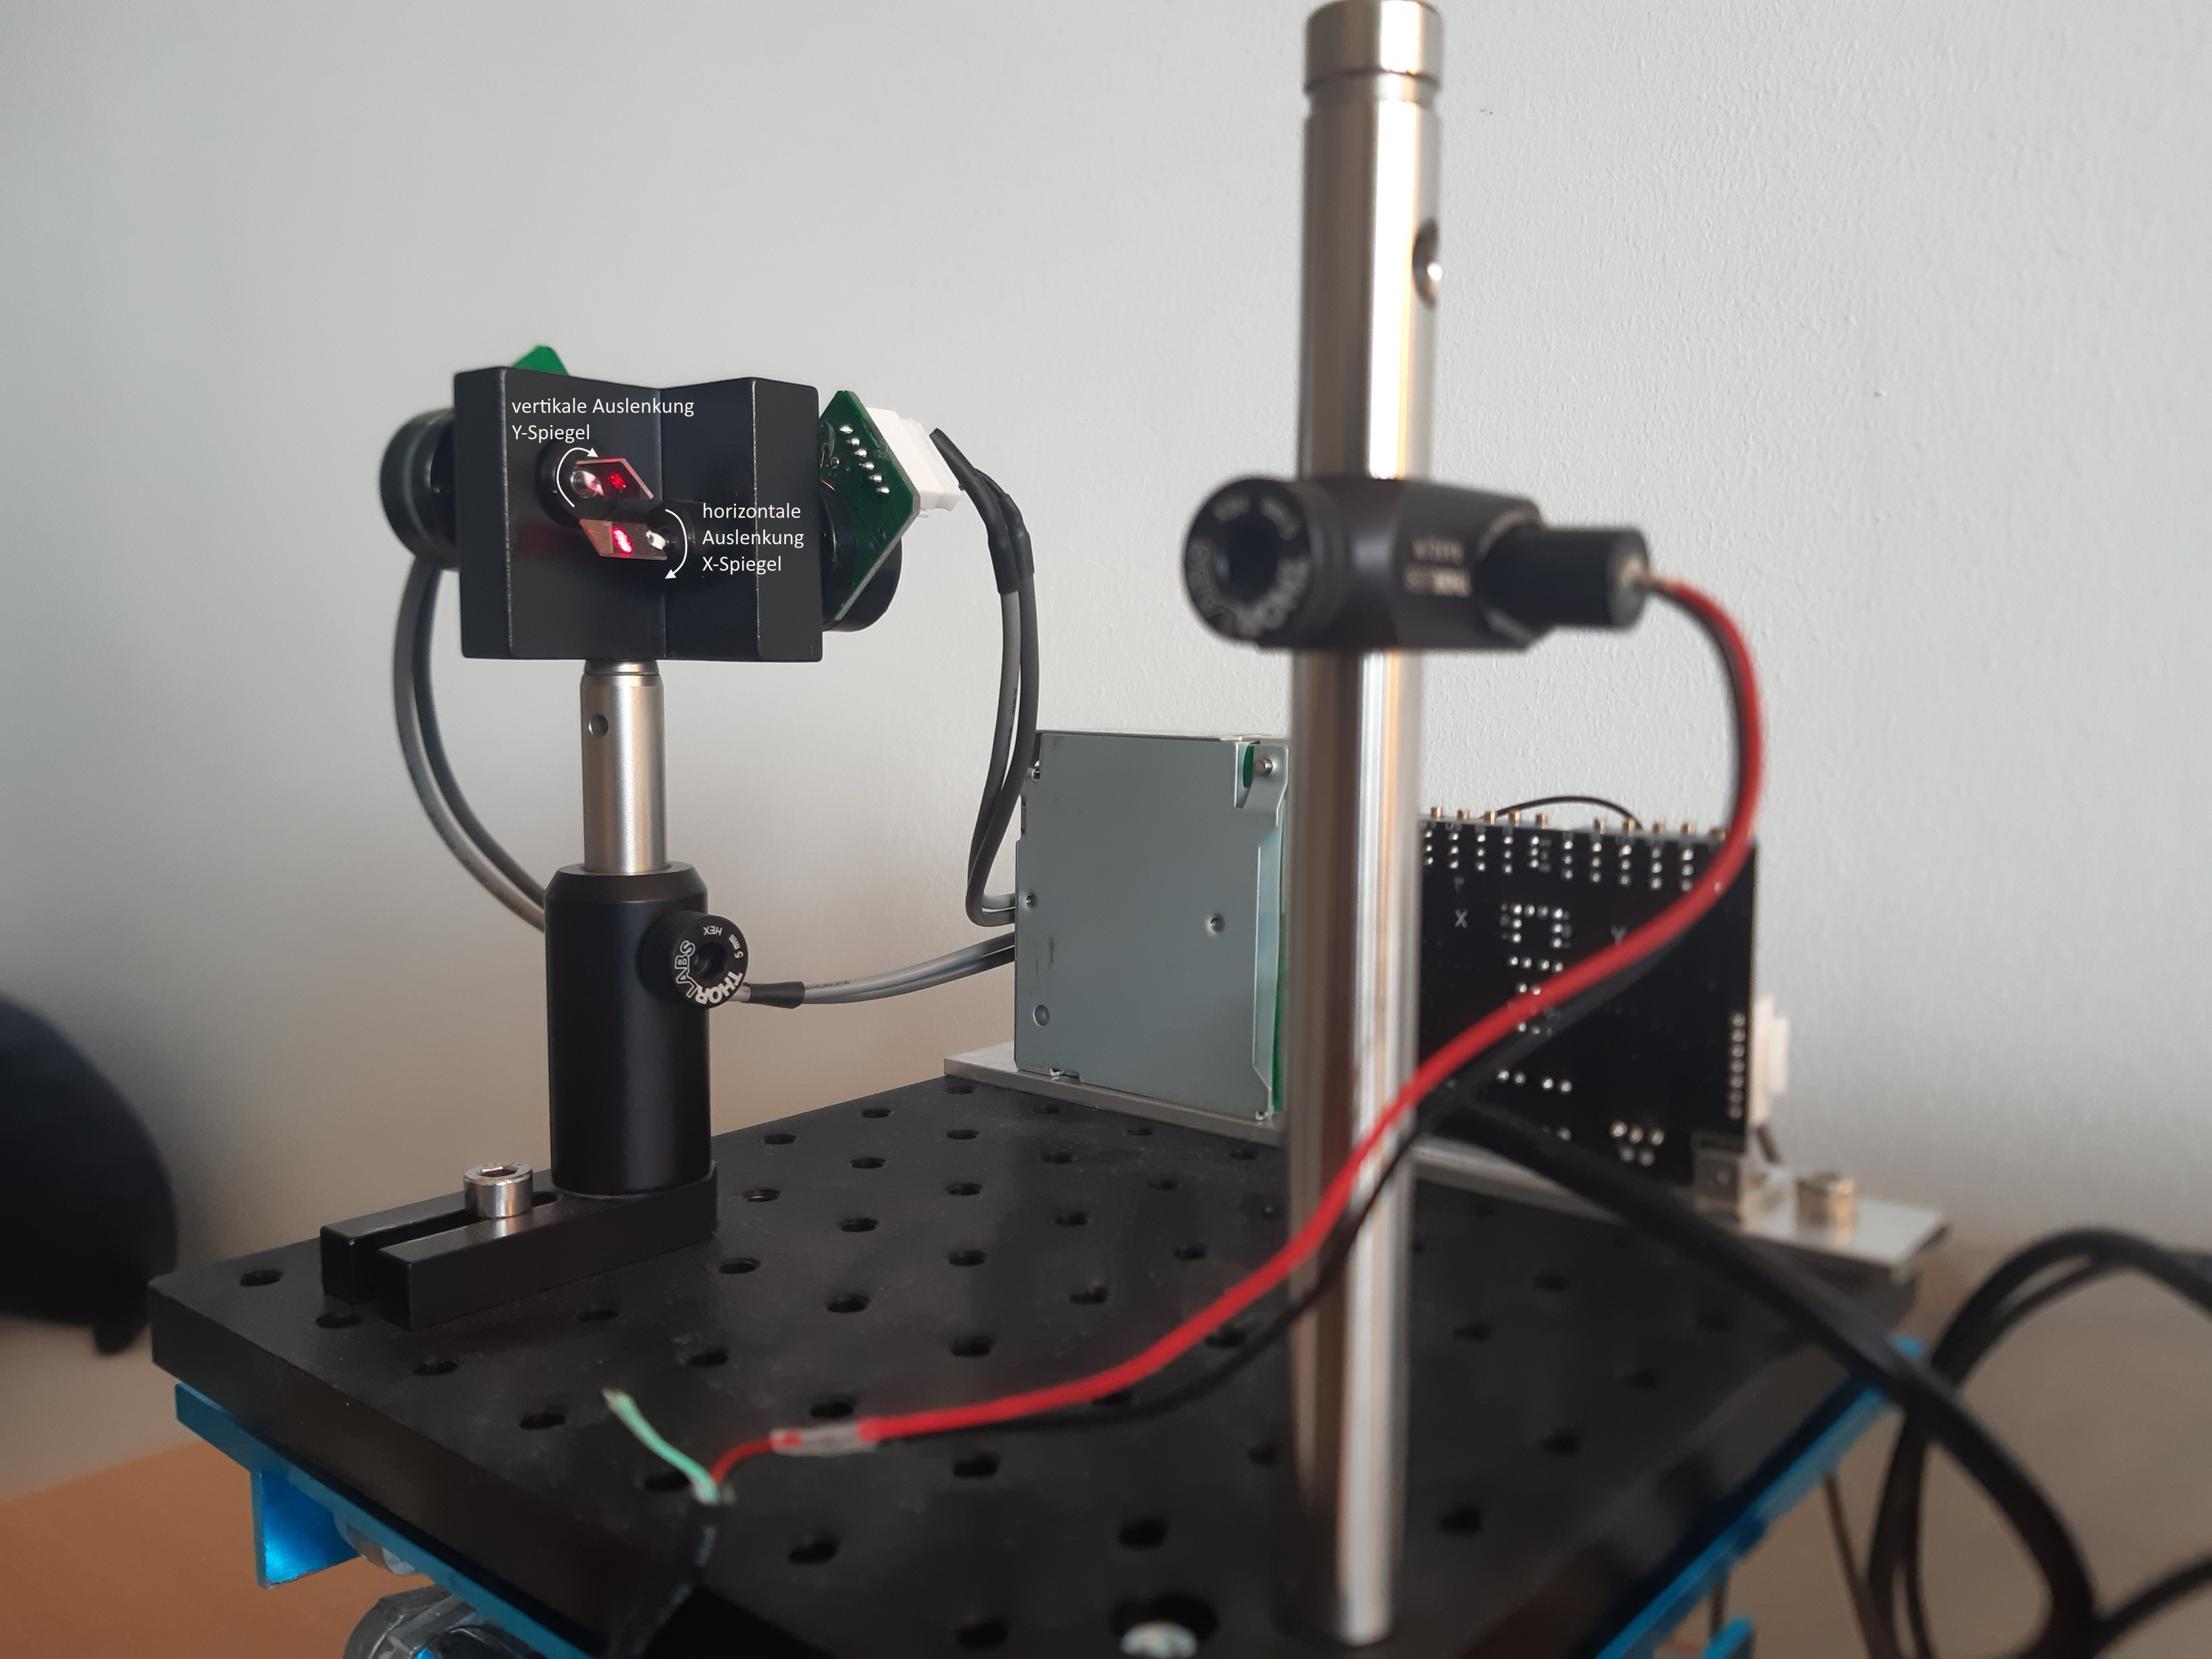
\includegraphics[width=\textwidth]{images/DetailGalvoOn.jpg}	\caption{DetailGalvoOn}	\label{DetailGalvoOn}	\end{figure}
\begin{figure}[h!]	\centering	\includegraphics[width=\textwidth]{images/DutTop02.jpg}	\caption{DutTop02}	\label{DutTop02}	\end{figure}

\section{Control of Galvanometer-Scanners}
Commercially available galvanometer scanners usually allow control in the form of analogue voltage inputs with a range of $\pm$ 10volts. The angle of the rotated mirror follows that control-voltage in a linear manner for sufficiently low frequencies. The signal-forms to result in the rectangular scan-grids, as described in the previous section, are depicted in fig.~\ref{GalvoRamps01}. To achieve these signals, a microcontroller-board was designed, including 16-bit analogue outputs, USB-connectivity and coaxial trigger outputs, among other features. To utilise these features and form an arbitrary signal generator for mentioned ramp-signals, a firmware is necessary. This should be done in a fashion employing quality-assurance during the implementation-process, as well as the verification-phase of the firmware and its supporting hardware. Aside from signal-generation and USB-connectivity, additional features are desirable, such as user-controllable relays, utilisation of watchdog-timer, UART-, I2C- and SPI-ports as well as analogue inputs. The combination of hard- and firmware will be called OCTane. Fig. ~\ref{blocktane} demonstrates the involvement of an OCTane into an OCT-system.
\bildGr{h!}{blocktane.pdf}{Integration of an OCTane}{blocktane}{0.75\textwidth}

\begin{figure}[h!]	\centering	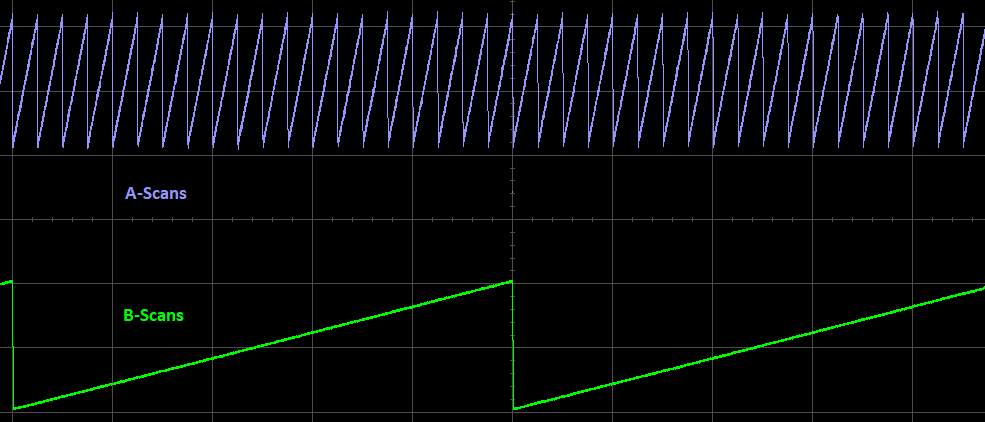
\includegraphics[width=\textwidth]{images/GalvoRamps01.png}	\caption{GalvoRamps01}	\label{GalvoRamps01}	\end{figure}
This leads to the scientific problem at hand: 
\begin{center} {\bf How can measures of quality be applied to a bare-metal firmware?}
\end{center}
% \subsection{optional: adapted steering curves}
% ...fliegt wohl raus
% \TODO{Modell ausm Paper per flachheitsbasierter Reglung auf Steuer-rampen draufrechnen}
% \textcolor{grey}{  }

% \TODO{"vom Allgemeinen zum Speziellen"}
% thethesis.tex
\chapter{Fundamentals - Code Quality and Real-Time}
\label{cha:Fundamentals}
	\section{Motivation}
	The areas of applications for microcontrollers, as well as the complexity of their software continues to grow. Also the demands towards correct and reliable function of those systems increase accordingly. Therefore software development requires significantly more effort than development of the corresponding hardware. As the lifespan of a software surpasses that of the corresponding hardware, these efforts becomes a sensible investment. To obtain the most value from that software-product, it has to fulfil certain quality measures. Neglecting these quality aspects would lead to an unjustifiable amount of work necessary for maintenance, when the product is already in service. Examinations of the dynamics of software development indicate, that, the later in a project lifecycle, changes become necessary, the higher the expenses. The worst case scenario: errors are induced in the implementation, persist unnoticed through testing and verification. Finally, this errors appear as faults in operation at the customer site. Furthermore, if the project suffers from lazy documentation and insufficient structure, identifying these errors and correcting them becomes even more expensive. The increasing complexity of nowadays software further escalates the problem. An even worse phenomenon can arise: Insufficient understanding of a faulty piece of software can lead to introducing even more errors with additional code, that is actually intended to fix a bug. Especially when poor structuring masks hidden dependencies between modules. A general rule of thumb is: The earlier an error originates, for example in the phase of gathering requirements, the more extensive changes are necessary, later on. In other words: The earlier an error is originates and the later it emerges, the more expensive are its consequences. Pursuing a sufficient quality level from the beginning of the project, significantly reduces waste of money, hours and enthusiasm on unnecessary maintenance. It may also substantially increase the customers approval \cite{Luo2001SoftwareTT}. % \TODO{Absatz}

	The described problems have suitable solutions. Applying the appropriate methods, implemented software can become reliable, easy to change, inexpensive to maintain and allow a more intuitive understanding. Distinguishable into two categories, these methods are either analytical or constructive. \\
	
	Best practice is to apply a circular combination of constructive and analytical methods. Constructive methods alone assist in preventing errors, but do not guarantee their absence. Analytical methods are capable of demonstrating the absence of errors, but not their prevention. Therefore a large amount of preventable errors might emerge, by exclusively applying analytical methods. The combined use consists of constructive methods during every phase of a development project, and assessing the intermediate results with analytical methods by the end of each phase. This process is called the "principle of integrated quality assurance" \cite{Liggesmeyer2002}. If the intermediate results do not meet the arranged quality criteria, the current state of the project does not reach the next phase, but remains in the extended current phase. This implies, that the current state of the product requires further development, until it fulfils all necessary quality criteria. This phase- and quality driven conduct, supports the development team in detection of errors at an early point and their removal at reasonable effort. Ideally, developers detect and eliminate all errors in the by the end of the same phase, where theses errors originate. This furthermore helps in minimizing the number of errors in a product over several phases. \\
	
	The described process makes it evident, that testing only a finished product is no sufficient way of ensuring high quality. Already the first intermediate result requires examination for deviations from the quality goals. Upon detection of deviations, measures have to be taken for correction at an early stage. Also an integration of constructive and analytical quality measures significantly improves the development process. While constructive methods are most helpful during the implementation activities of a phase, the corresponding assessment benefits primarily from analytical measures. \\
	
	A further incentive in testing, especially in the formal way of well defined test-cases, originates from Boris Beizers quote from "Software Testing Techniques" \cite{Beizer90}:  
	\begin{quote}
	The act of designing tests is one of the most effective bug preventers known % 
	\end{quote}
	Additionally to the safeguarding of existing functionalities and helping in detecting errors, the thought process of formal testing methods also helps in better understanding and developing of software. \\

	The early definition of quality goals is a key factor, as it allows to achieve the intended quality. It constitutes of the specification of the desired quality features, not of defining the software requirements. This has to happen even before the phase of requirement-definition, as the requirements themself are affected by aforementioned quality goals. On the other hand, testing results against quality features is also of vital importance. \\ 
	
	The typical approach of developers is, to test a program in its early stages. This is already an informal dynamic test. Inspecting the code after implementation for structural errors is the informal equivalent of a static analysis. Application of these informal methods is very common, while formal processes of testing is much less established. Ideally, testing generates reproducible results, while following well defined procedures. \\

	While hardware quality assurance often results in quantitative results, this is usually not the case for software. But processes exist for both worlds, to ensure systematic development, as well as quality assurance. Developers of systems integrating both hardware and software have to be aware of their differences. Combining the quality measures for soft- and hardware allows to consider interactions between soft- and hardware. This prevents interactions to corrupt quality goals. Developers have to specify and verify quality properties for the complete system. It is insufficient to perform this tasks on separate modules. The correct behaviour of the whole system requires demonstration, as the test results of individual modules, usually, can not be superimposed.
	
	% \TODO{... bis hier nach Langer-Review korrigiert}
	\section{Terminology and Definitions of Terms}
	To clarify regularly used terms, here are definitions in accordance with either \cite{Kopetz1997} or \cite{Liggesmeyer2002}
	\subsubsection{Quality, Quality Requirements, Quality Features, Quality Measures}
		\begin{itemize}
		\item Quality, according to the standard 'DIN 55350 - Concepts for quality management', is defined as: The ability of a unit, or device, to fulfil defined and derived quality requirements.
		\item Quality requirements describe the aggregate of all single requirements regarding a unit or device.
		\item Quality features describe concrete properties of a unit or device, relevant for the definition and assessment of the quality. While it does not make quantitative statements, or allowed values of a property, so to say, it very well may have a hierarchical structure: One quality feature, being composed of several detailed sub-features. A differentiation into functional and non-functional features is advised. Also features may have different importance for the customer and the manufacturer. Overarching all these aspects, features may interfere with each other in an opposing manner. As a consequence, maximizing the overall level of quality, regarding every aspect, is not a feasible goal. The sensible goal is to find a trade-off between interfering features, and achieve a sufficient level of quality for all relevant aspects. Typical features, regarding software development include: Safety, security, reliability, dependability, availability, robustness, efficiency regarding memory and runtime, adaptability portability, and testability.
		\item {Quality measures} define the quantitative aspects of a quality feature. These are measures, that allow conclusions to be drawn about the characteristics of certain quality features. For example, the MTTF (mean time to failure), is a widespread measure for reliability.
		\end{itemize}
	
	\bildGr{b!}{ErrorFaultFailure.pdf}{Causal chain of failures.}{ErrorFaultFailure}{0.5\textwidth}

	\subsubsection{Error, Failure, Fault}
	\begin{minipage}{\linewidth}
	\begin{itemize}
		\item {Error}, the root cause of a device or unit to fail, may originate from operation outside the specification, or from human mistakes in the design.
		\item {Failure}, or defect is the incorrect internal state of a unit, and is the result of an error. It exists either on the hard- or software-side and is the cause of a fault, but not necessarily.
		\item {Fault} is the incorrect behaviour of the unit, or it's complete cease of service, observable by the user. It is caused by a failure.
		\item These definitions are in accordance with \cite{Liggesmeyer2002} and \cite{Kopetz1997} and have causal dependencies, depicted in Fig.~\ref{ErrorFaultFailure}.
		\item While an error can be classified by its persistence, being permanent or transient, failures and faults are classified more detailed into consistent/inconsistent, permanent/transient and benign/malign, among other categories.
	\end{itemize}
	\end{minipage}
	
	\subsubsection{Correctness}
		{Correctness} is the binary feature of a unit or device, loosely described as 'the absence of failures'. A more specific description would be, that a correct software operates consistent to its specification. This implies, that no conclusion about correctness is possible, without an existing specification.
	\subsubsection{Completeness}
		{Completeness} describes, that all functionalities, given in the specification are implemented. This includes normal intended operation, as well as the handling of error-states. It is a necessary, but not a sufficient criterion for correctness.
	\subsubsection{Testability}
	{Testability} describes the property of a unit, to include functionality dedicated only to facilitate the verification of that unit. Supporting concepts include the \\
	% \begin{minipage}{\linewidth}
	\begin{itemize}
		\item Partitioning of the whole unit into modules, that are testable in isolation. These modules should have little to no side-effects with each other. 
		\item A dedicated debug-unit, making the actual state of the unit observable from outside further assists Testability. 
		\item Another concept is, to specify only as much input space as is necessary, resulting in fewer necessary test-cases to ensure a high coverage.
	\end{itemize}
	% \end{minipage}

	The aggregate of these concepts is called {\bf design-for-testability}.
	Generally, time-triggered units support testability to a higher degree, than event-triggered systems.
	\subsubsection{Safety and Security}
	% \begin{minipage}{\linewidth}
	\begin{itemize}
		\item {\bf Safety} means, that a unit is fit for its intended purpose and provides reliable operation within a specified load- and fault-hypothesis.
		\item {\bf Security}, though, is the resistance of unit against malicious and deliberate misusage.
	\end{itemize}
	% \end{minipage}
	\subsubsection{Reliability}
	{Reliability} is a dynamic property, giving the probability, that a unit is operational after given time {\bf t}.
		\begin{align*}
		\textrm{Reliability ...} \quad R(t) & = e^{-\lambda (t-t_o) }\\
		\textrm{failure rate ...}  \quad \lambda & = \frac{1}{MTTF} 
		\end{align*}
	An exponential function, decaying from 100\% at time = t0, where a unit was known to be operating. $\lambda$ is the failure rate with dimension 'failures/h'
	
	\subsubsection{Maintainability}
	{Maintainability} is the probability, that a system is repaired and functioning again within a given time after a failure. Note that this includes also the time required to detect the error.
	A quantified measure for it is the mean-time-to-repair (MTTR).
	\subsubsection{Availability}
	{Availability} combines reliability and maintainability into a measure, giving the percentage of time, a unit is operational, providing full functionality.
		\begin{align*}
	\textrm{Availability ...} \quad A & = \frac{MTTF}{MTTF + MTTR}
		\end{align*}
	It is apparent, that a low time-to-repair and a high time-to-failure leads to high availability.
	\subsubsection{Robustness}
		Robustness is actually a property of the specification and requirements. While correctness rates, how far the implemented software complies with the specification, it correct software still might fail in critical situations, that are not covered in the specification. Therefore, to achieve robustness, the specifications have to be examined and ensured, that all critical situations are covered and the expected behaviour of the device under these conditions is defined.
	\subsubsection{Dependability}
	{Dependability} finally, is composed of sufficiently fulfilled levels of \\
		% \begin{minipage}{\linewidth}
		\begin{itemize}
			\item Reliability
			\item Availability
			\item Maintainability
			\item Safety
		\end{itemize}
		% \end{minipage}
	...assembled into the common acronym {\bf R.A.M.S.}
	
	% \subsection{load-hypothesis, fault-hypothesis}
		% \TODO{Erklärung} 
		
	\subsection{Bare Metal-Systems}
	The label 'bare-metal system' applies to firmware that does not contain an operation system. Various components may be present, for example I/O-device management and a user-interface are indispensable. Nevertheless, a kernel and process management are not part of a bare-metal system, also a file-system is rather uncommon. This comes with various implications, as this forces developers to cross-compile their code on a different system. Furthermore, initializations of hardware-components and peripherals, scheduling of phase-sensitive tasks and handling of interrupts has to be implemented by a developer, instead of delegating these duties to an operation-system.
	
	% \section{Code Quality}

	\section{Function-oriented Testing}

	This chapter establishes methods to design test-cases, to verify a given piece of software against its specification. The first method, named 'equivalence partitioning', assists in reducing all possible inputs to an examined unit, down to a sufficient set of inputs, while the second method 'state based testing' aims to sufficiently cover code, whose behaviour relies heavily on its own condition and history. Both are best suited in a white-box scenario, that means, that the inner structure of the examined software must be known to the tester, for example in form of the not compiled source-code. Equivalence class partitioning might be applied in a black-box scenario, where only a specification is present, but the consequential flaws of such an approach will become apparent in the following chapter.

	\subsection{Equivalence Class Partitioning}
	This method is applied most beneficial on a unit- or module level testing. The input- and output spaces of various functions might allow an extreme amount of values, testing them all would lead to unacceptable amount of test-cases and would prevent their execution in a feasible time. Then again, many of those possible inputs would take the same paths through the examined module, in other words, excite the module to the same behaviour. Such a sub-set of inputs forms a common class, a so called 'equivalent class', that can ideally by represented by one input and therefore one test-case. A distinction of cases inside a module would form separate paths for the information to take, therefore form different behaviours of the module itself. Each of those distinctions call for a separate equivalence class and their own test-case. The aggregate of test-cases to cover all possible paths through a unit, or to trigger all possible kinds of behaviour of a unit, form a sufficient set for function-oriented testing. This method, that applies the ancient concept of 'divide and conquer', partitions a unit into low levels of complexity, that can be represented by one single equivalent test-case, thus giving it the name 'equivalence partitioning'.

	Equivalence classes should initially be derived from the software's specification and can be distinguished into input- and output-classes. While forming a specific output-class it shall be noted, that an according choice of input values has to be defined, presumably exciting the tested unit to the desired or specified output values. \\
	An equivalence class, representing valid input or output values is hence called 'valid equivalence class'. For input or output values, that are specified as invalid, or not specified at all, according 'valid equivalence classes' must be formed as well, to test a units capability in handling those exceptional situations and possibly reveal errors inside a unit. This differentiation in types of test-classes is illustrated in Tab. ~\ref{EquiClasses}.
	
	\begin{table}[h!]
	\begin{center}
		\begin{tabular}{c c}
		
						& port-wise  \\
		validity-wise	& \begin{tabular}{|c | c|} \hline
						valid input class 	& valid output class   \\  \hline
						invalid input class 	& invalid output class \\ \hline
							\end{tabular}		\\ % \hline 
		\end{tabular}
			\caption{Distinguishing equivalence classes.}
			\label{EquiClasses}
	\end{center}
	\end{table}
	While output classes are much less common in everyday programming, their importance shall not be neglected: Identical inputs might very well result in different outputs, depending on varying side-effects, that have influence on the inspected unit. This has to be accounted in separate equivalence classes for expected outputs.
	
	Following this first steps of partitioning, the resulting classes shall further be separated into sub-classes that take into account distinction of cases within a module, where data might travel several different paths or branches of the source code. This step is only possible in a white-box-scenario, as it requires direct inspection of the source-code. While demanding additional effort, this allows to examine also rather hidden corners of the source-code, that otherwise might go unnoticed and possibly mask hidden errors.

	Some examples demonstrate the correct application of the described method:
	

	\begin{itemize}
		\item valid/invalid input classes: \\
			input is specified as an integer number between 1 and 20 volts \\
			$\rightarrow$ valid class: 1 $\le$ 'test-value' $\le$ 20 \\
			$\rightarrow$ invalid class: 1 > $test-value$ and \\
			$\rightarrow$ invalid class: <test-value> > 20 \\
		\item output class: \\
			output is specified for given input filenames as: 0 if file exists, -1 if file does not exist. \\
			$\rightarrow$ valid class: Filename of an existing file\\
			$\rightarrow$ invalid class:  Filename of an inexistent file\\
			$\rightarrow$ invalid class:  String with a malformed file-path \\
		\item dedicated allowed values: \\
			addressed module can be chosen from TriggerA, TriggerB, or TriggerC. \\
			$\rightarrow$ valid class: TriggerB \\
			$\rightarrow$ invalid class:  TriggerK \\
			$\rightarrow$ invalid class:  Trucker \\
		% \item in-source:
			% Aus einer bekannten IF-Schleife werden zwei TCs
	\end{itemize}

	A visual explanation of the first example is given in Fig. ~\ref{EquivPart01} 
	\bildGr{h!}{EquivPart01}{Basic equivalence partitions.}{EquivPart01}{\textwidth}
	
	\subsection{Boundary Value Analysis} %  (Grenzwertanalyse, Ligges)
	Until now it might seem, that test-values can be chosen randomly from gathered classes, which is often a sufficient case. But a closely related method called 'boundary value analysis' refines the selection of test-values. From a set of integers between 10 and 100, with a known code structure to be free from case distinctions, the representative test-value can truly be chosen randomly as 15, 60, or 78. In more complex numerical structures, like floating-point numbers, overarching '0' and negative numbers as input space, a single value becomes insufficient. It is then advisable to deliberately choose values close to the bounding values of a function and in the given case also values close to the '0'.
	Further explanation of choosing useful values will be given on a slight variation of the first equivalent classes-example: Assumed is a function specified for floating point input values in the range of $\pm$ 10V. 
			\bildGr{h!}{EquivPart02}{Equivalent class for floating-point numerical input.}{EquivPart02}{\textwidth}
	The given set, visualized in Fig. ~\ref{EquivPart02}, has obvious bounding values of +10 and -10, giving the first to test-values. Small values deviating from $\pm$ 10V are also values to test for. Furthermore, '0' and small values deviating from 0 in positive and negative direction will reveal the units stability, in case, the input is used as a divisor. \\
	This results in the following classes and their according values for test-cases:
	\begin{align*} % \setlength\itemsep{1px}
	0.00		& \rightarrow   Test-Case 1		 \\
	10.00		& \rightarrow   TC2	 \\
	-10.00		& \rightarrow   TC3	 \\
	-0.01		& \rightarrow   TC4	 \\
	0.01		& \rightarrow   TC5	 \\
	9.99		& \rightarrow   TC6	 \\
	-9.99		& \rightarrow   TC7	 \\
	10.01		& \rightarrow   TC8	 \\
	-10.01		& \rightarrow   TC9	 \\
	\end{align*}
	And their categorization into valid/invalid values:
	\begin{itemize}[label={}]
		\item	$\rightarrow$ valid classes: +10V, +9.99V, -10V, -9.99V, 0V, +0.01V, -0.01V \\
		\item	$\rightarrow$ invalid classes: +10.01V, -10.01V \\
	\end{itemize}


	
	Every value has to be applied via a separate testcase, to alleviate which values cause problems, in case of failing tests. \\
	Boundary value analysis and equivalence class partitioning are closely related and often mentioned in unison, nevertheless, their separate description in this chapter is intended to specify their different applications.
		
	% \subsection{State Based Testing}

	% Darauf hat PlagAware angeschlagen, engl Präs vom Ligges:
	% technodocbox.com/C_and_CPP/94907983-Software-quality-assurance-dynamic-test.html
	

\pagebreak	
	% von Josef abgesegnet
	\section{Coverage Metrics}
	Code coverage belongs to the group of dynamic testing techniques, and concerns itself with the structure of software. It is part of the class of control-flow and structure-oriented dynamic testing techniques. The primary application of this white-box technique lies in testing modules and units, thus 'testing on a small scale'. On the level of integration-tests, coverage has valid applications and is rather common among developers. There is contradicting literature, whether or not code coverage is a suitable technique on a system level of testing (see \cite{Tian2005} vs. \cite{Liggesmeyer2002} ) \\
	The term 'coverage' refers to the amount of source code, a program executes and therefore 'covers', during testing. Covered code delivers results that require assessment of their correctness against a specification. Uncovered code requires additional test cases ensuring coverage of those areas. Code coverage allows the combination with other test techniques, that describe the generation of those test cases, because code coverage does not specify rules for that. \\
 	
	The following list shows control-flow-oriented techniques, relevant for this thesis:
	\begin{itemize} \setlength\itemsep{1px}
		\item Statement coverage
		\item Branch or decision coverage
		\item Basic condition coverage
		\item Condition/decision coverage
	\item Boundary-interior coverage, structured path test
		\item Modified condition/decision coverage (MCDC)
		\item Modified boundary-interior test
		\item Path coverage
		\item Multiple condition coverage
	% \item ( State and transition coverage ) % Tian S.153
		\item Mutation analysis \\
	\end{itemize} 

	Fig. ~\ref{SubsumptionHierarchy01} demonstrates the implicative relations of the coverage types in aforementioned list. For example, complete decision coverage implies	full statement. Multi-Condition and path coverage on the other hand have no relevant relation to each other and both constitute the strongest coverage metric in their own aspect. \\
	
	\bildGr{h!}{CoverageSubsumption.pdf}{Subsumption hierarchy of software testing methods \cite{Liggesmeyer2002}.}{SubsumptionHierarchy01}{0.49\textwidth}
	% \bildGr{h!}{CoverageSubsumption.png}{Subsumption Hierarchy}{SubsumptionHierarchy02}{0.75\textwidth}

	Statement coverage is the most basic metric and only requires to execute every line of code, existing in the code under test. A sufficient amount of test-cases should always achieve 100\% statement coverage, otherwise 'unreachable' code sections indicate design-flaws. \\
	
	Branch or decision coverage indicates, if a program executes all branches. It subsumes statement coverage and extends the concept, in that, every decision in the source code must evaluate to true and false. A decision is possibly composed of multiple elementary or atomic conditions. \\
	
	Basic condition coverage indicates, if all elementary conditions evaluate to both possibilities. It requires, that in compound decisions, every elementary condition separately results to true and false.  \\

	Condition/decision coverage consists of all requirements from basic condition coverage and branch or decision coverage combined. It is a relevant metric in case of complete evaluation of compound decisions, in contrast to short-circuit evaluation. It subsumes statement, branch or decision and basic condition coverage. \\
	
	Boundary-interior coverage is a metric for the sufficient testing of loops, while the structured path test describes, how to design corresponding test-cases. It requires separate test-cases that enter a loop, with (interior) and without (boundary) incrementing it.	Because of these special requirements, it cannot be subsumed by previous metrics. Therefore, it resides in a separate branch of the hierarchy-tree in fig. ~\ref{SubsumptionHierarchy01}. \\

	Modified condition/decision coverage (MC/DC) is a refinement of condition/decision coverage. It requires every elementary condition to result in true and false. Additionally, it  demonstrates the impact on the compound decision, separately for every elementary condition. 	\\

	The modified boundary-interior test is similar to the structured path test, but requires separate test-cases for every loop, especially nested loops. Paths, that execute a loop and vary in the execution of nested loops, count as one path. Paths that only vary outside the examined loop do not require separate consideration. Finally it explicitly requires complete branch coverage, regardless of the previous rules. \\

	Path coverage refers to the execution of all possible paths, present in the code under test. It is the strongest requirement towards evaluation of program-flow and subsumes boundary-interior coverage as well as the modified boundary-interior test.  \\

	% bis hierher von Josef abgesegnet

	Multiple condition coverage extends basic condition coverage, by imposing the strongest requirement towards compound decisions: Every possible result of one elementary condition, true or false, has to be combined with every possible result of every other elementary condition. \\

	% \item Partition coverage
	% State and transition coverage indicates which states and transitions a given finite state machine executes.  \\ % Tian S.153

	Mutation analysis deliberately manipulates the code under test to demonstrate, whether the present test-cases detect these changes. It is an auxiliary method to assess capabilities of test-cases, though not a type of coverage itself. \\

	The major similarity of all coverage types, is the intention to indicate the completeness of the code under test, albeit with regards to different aspects. Also, they all strive to execute all possible variants of decisions, branches and parameter spaces. This aims to reveal all possible errors, as software under execution will either show the intended or divergent behaviour. In the latter case, measures to eradicate found errors during development are necessary. A lack of coverage indicates insufficient testing, while not every metric allows to achieve 100\% coverage in practicable time. Adding test-cases is a feasible way to improve coverage. Branches, decisions or statements, that no sensible test-case can reach, suggest a flaw in the software design. \\

	\subsubsection{Limitations}
	The most prominent limitation of any type of coverage lies in the aspect, that it can exclusively test, what is implemented: Coverage can not reveal functionalities, that are part of the Specification, but do not have an Implementation. \\	
	Furthermore, the higher ranking a type of coverage, the more difficult it becomes, to achieve complete coverage. In this context, a higher level in fig. ~\ref{SubsumptionHierarchy01}  indicates a higher ranking coverage. While a complete statement coverage is a minimal criterion for sufficiently testing a program, same is not the case for the more complex types of coverage. \\

	In many cases it is neither possible nor necessary, to test every path or combination of conditions. Nonetheless, In these situations, the according coverage metric is useful in pointing out 'unreachable' states of the program. It is then upon the developer to interpret the coverage report. If it indicates a design flaw, changes to the program are necessary. If the report points out states in the program that are reliably unreachable, neither during testing, nor during execution, the responsible developer may decide these states to be 'not worthy of testing'. Nevertheless, this requires to profoundly argue such a decision, communicate it all affected team-members and documented it. Lastly, reports of uncovered states can be useful as hints, to construct complexer test-cases to also cover these states. \\

	\subsubsection{Control-flow Graph}
	The basis for all control-flow oriented tests is the control-flow graph. Fig. ~\ref{ctrlFlowExamp} shows an example of a simple function, containing a loop and an if-condition. This graphical representation visualizes, in an intuitive way, which paths can be traversed during execution of a delimited piece of code. To maintain clarity in the resulting image, a single graph should only visualize small parts of a program, typically a single function. Larger amounts of code rapidly lead to overwhelmingly complex control-flow graphs. This type of graph is able to represent any program, written in an imperative programming language. \\
	
	\bildGr{h!}{ctrlFlowExamp}{Example of a control flow graph of a looped function.}{ctrlFlowExamp}{0.35\textwidth}
	The following sections offer more detailed descriptions of coverage metrics.
	\subsection{Statement Coverage Test}
	The basic control flow oriented test method is the statement or line coverage, also known by the abbreviation C$_0$. It aims to execute every statement, or line of code, at least once. Regarding the control flow graph, this means to execute every node of the graph. The definition of this metric is the amount of executed code versus the amount of existing code:
		\begin{align*}
		C_0 = \frac{\textrm{number of executed statements}}{\textrm{number of statements}}
		\end{align*}
	Usually, coverage reports state this and similar metrics in percent. 100\% or complete statement coverage denotes the execution of every line of code at least once. One obvious benefit lies in the immediate detection of non-executable code sections, also known as 'dead code'. Another benefit lies in revealing possible errors, present in the tested code: Incomplete statement coverage encourages a developer to add test-cases, to execute and test also the remaining areas of code. If their execution triggers an existing error, this error becomes apparent by causing either faulty output or even a crash of the program. And only after an error becomes apparent, a developer can apply counter-measures against it. \\
	This ability of the statement coverage is limited to errors, that are sensitive to execution, regardless of input. This metric only requires to execute code and does not specify, which input values to apply. Furthermore, conditional execution has only minor impact on statement coverage, so if- case- and loop-statements do not undergo thorough examination. \\
	In general, statement coverage is usually a by-product of other coverage metrics and not determined via an independent test procedure, because many other coverage metrics imply the statement metric. Nevertheless, as basis for most higher-level coverage metrics, statement coverage is still worth studying and understanding. Because of the inherent shortcomings, it is a necessary, but not sufficient metric for adequate software testing. \\
	\subsection{Branch or Decision Coverage Test}
	% conditional
	The branch coverage, also called decision coverage, concerns itself with the conditional execution of code. It is a more advanced method than the statement coverage and represents the minimum criterion in control-flow oriented testing. Again, regarding the control flow graph, this means to traverse every edge of the graph. \\ Obviously, statement coverage does not guarantee the execution of every branch, as nodes may have multiple edges leading to and from them. The example in fig. ~\ref{ctrlFlowExamp} contains an edge to the very right, that would require traversal for branch coverage, but may be ignored by statement coverage. The alternative label 'decision coverage' refers to the inherent requirement, that every decision must at least once result to 'true' or 'false' \cite{Tai1980ProgramTC}. \\
	Branch coverage goes by the abbreviation $C_1$ and measures the amount of executed branches versus the amount of existing branches, again in percent.
		\begin{align*}
		C_1 = \frac{\textrm{number of executed branches}}{\textrm{number of branches}}
		\end{align*} \\
	% https://www.cs.odu.edu/~zeil/cs333/website-s12/Lectures/wbtesting/pages/gcov-branch.html
	% gcov flags:
	  % -b, --branch-probabilities
	  % -c, --branch-counts	
	Based on its definition, branch coverage is able to quantify the execution of branches and draw conclusions upon the resulting categories. \\
	\begin{itemize} \setlength\itemsep{1px}
	\item not executed branches
	\item seldom executed branches
	\item often executed branches \\
	\end{itemize} 

	On the one hand, not executed branches may turn out to be unnecessary, signify a design error and could be eliminated. On the other hand, it can indicate, that preconditions to reach a branch are difficult to generate via test-cases. The test report may then contain hints towards the design of suitable test-cases. Often executed branches represent candidates for optimization. Speeding up code, that is run very often is, obviously, more beneficial, than optimizing code that executes rather seldom. \\

	Drawbacks of branch coverage contain insufficient assessment of loops, as this metric only requires to execute a loop-body once, regardless of loop-counters. Also not all possible combinations of edges within the control-flow graph have to be traversed. This may hide errors that would emerge only upon traversal of very specific execution paths. These special paths are not necessarily contained in test-cases, that would otherwise suffice for branch coverage. Furthermore, compound conditions are not reviewed in detail. \\

	\subsection{Basic Condition Coverage Test}
	The next more sophisticated metric is the (Basic) Condition coverage. It extends the concept of branch coverage, by closer examination of compound or composite conditions. The terminology regarding abbreviation is not consistent for this and the following types of coverage. Some sources denominate condition coverage as $C_2$, while other sources attribute the same symbol for the structured path test. Therefore, this thesis omits further examples of that notation. \\
	Fig. ~\ref{compDecision} gives an example of such a condition. 
	
		% \bildGr{h!}{compDecision}{Example of a compound condition.}{compDecision}{0.75\textwidth}
		\bildGr{h!}{compDecision01}{Example of a compound condition.}{compDecision}{0.75\textwidth}
	
	Condition coverage requires every separate elementary decision to result in 'true' and 'false', while branch coverage demands this only for the complete condition. In particular, condition coverage demands, that 
	\begin{itemize} \setlength\itemsep{1px}
		\item \lstC |	strPtr != NULL 		|
		\item \lstC | 	isObsolete(strPtr)	| and
		\item \lstC | 	isValid(strPtr) )	|
	\end{itemize}
	have to result to 'true' and 'false', independently. \\

	In the usual case of short-circuit evaluation, the if-condition can possibly leave out execution of second or third arguments at all. In the given case, the subroutine \lstC ! isOsbolete(strPtr) ! is not guaranteed to undergo execution, would it be not deliberately required by condition coverage. The developer might force the compiler to abstain from short-circuit evaluation and therefore achieve the execution of every single argument. Nevertheless, the thorough way, is to design separate test-cases, aiming for the examination of elementary decisions. This is because during debugging, separate test-cases indicate the source of failure within a compound condition more specific, than just one test-case for the whole condition. Furthermore, complete evaluation would prevent condition coverage, to completely subsume branch coverage. \cite{Kalkov2013CodeCC}
	
	Condition coverage, partially, considers the complexity of compound conditions, which is neglected by decision coverage.
	
	\subsection{Condition/Decision Coverage Test}
	Condition/Decision Coverage extends the requirements of the basic condition coverage, by literally demanding the execution of every branch. As described earlier, this is not guaranteed by basic condition coverage, in case, the compiler performs complete evaluation. For reasons already described, this thesis only considers short-circuit evaluation. In this case, condition/decision coverage and basic condition coverage become identical.

	A common weakness of both these metrics lies in only dissecting compound conditions into its elementary decisions. While this addresses problems arising from short-circuit evaluation, it does not regard inter-dependencies between elementary decisions.
	
	\newcommand{\mcdc}{MC/DC }
	\subsection{Modified Condition/Decision coverage test (\mcdc)}
	The modified condition/decision coverage targets nested logical links between elementary decisions and is abbreviated '\mcdc'. It achieves this by demanding to demonstrate every single elementary decisions impact on the compound condition, independently. This is not guaranteed by condition/decision coverage. It is a thorough method to examine compound conditions, at reasonable effort. This is due to the linear relation between the complexity of a compound condition and the test effort: According to \cite{ChilenskiMiller1994} \mcdc requires N+1 test-cases to comprehensively assess a compound condition containing N elementary decisions. \\

	Tab. ~\ref{MCDCtable} demonstrates the possible combinations of four elementary decisions for the compound condition \lstC !(A||B)\&\&(C||D)! .

	\begin{table}[h!]
		\begin{center}
			\begin{tabular}{c|c|c|c|c|c|c|c}
			Testcase & A 	& B		& C		& D		& A||B	& C||D	& (A||B)\&\&(C||D)	\\ \hline
			1		 & 0 & 0	& 0	& 0	& 0	& 0	& 0	\\ \hline
			2		 & 0	& 0	& 0	& 1 	& 0	& 1	& 0	\\ \hline
			3		 & 0	& 0	& 1	& 0	& 0	& 1	& 0	\\ \hline
			4		 & 0	& 0	& 1	& 1 	& 0	& 1	& 0	\\ \hline
			5		 & 0	& 1	& 0	& 0	& 1	& 0	& 0	\\ \hline
			6		 & 0	& 1	& 0	& 1 	& 1	& 1	& 1	\\ \hline
			7		 & 0	& 1	& 1	& 0	& 1	& 1	& 1	\\ \hline
			8		 & 0	& 1	& 1	& 1 	& 1	& 1	& 1	\\ \hline
			9		 & 1	& 0	& 0	& 0	& 1	& 0	& 0	\\ \hline
			10		 & 1	& 0	& 0	& 1 	& 1	& 1	& 1	\\ \hline
			11		 & 1	& 0	& 1	& 0	& 1	& 1	& 1	\\ \hline
			12		 & 1	& 0	& 1	& 1 	& 1	& 1	& 1	\\ \hline
			13		 & 1	& 1	& 0	& 0	& 1	& 0	& 0	\\ \hline
			14		 & 1	& 1	& 0	& 1 	& 1	& 1	& 1	\\ \hline
			15		 & 1	& 1	& 1	& 0	& 1	& 1	& 1	\\ \hline
			16		 & 1	& 1	& 1	& 1 	& 1	& 1	& 1	\\ \hline
			\end{tabular}
			\caption{Test-cases for \mcdc coverage.}
			\label{MCDCtable}
		\end{center}
	\end{table}
	% \newpage
	Following the rule, to demonstrate each elementary decisions impact on the compound condition, only the test-cases number 2, 6, 9, 10 and 11 are necessary. This amounts to five test-cases, which equals the number of elementary decisions+1. \\
	Considering logic dependencies among elementary decisions can reduce the number of test-cases, even more. The decision in fig. ~\ref{compDeciMutualEx} implies a truth-table similar to tab. ~\ref{MCDCtable}, but with $2^{5} = 32$ entries or lines. Obviously, the left input operand is identical in all five elementary decisions. Therefore, those elementary decisions are mutually exclusive, as, for example, col can not be RED and BLUE at the same time. This leads to the conclusion, that only five test-cases with valid input values and one invalid test-case are necessary. In this case, six test-cases are sufficient for \mcdc coverage instead of 32. The similarity of this example with a 'switch-case' statement suggests, to apply \mcdc also to this kind of selection control mechanism \cite{Chilenski2001}. \\
	\bildGr{h!}{compDeciMutualEx}{Mutual exclusive example of a compound condition.}{compDeciMutualEx}{\textwidth}
	Although, this chapter puts emphasis on the design of suitable test-cases, \mcdc does not provide specifications for that. It is due to the lack of free and mature software tools to measure \mcdc coverage of C-code on a bare-metal system. Therefore, the guidelines to produce test-cases aim to counter that lack. \\

	The advantage of the \mcdc, evidently, lies in the thorough test of compound conditions with feasible effort. For a condition, composed of four elementary decisions, only five of sixteen possible input combinations require test-cases. It implies all aforementioned coverage metrics \cite{Hayhurst2001APT}. \\
	
	The described advantages come at the price of higher efforts in identifying suitable stimuli as test-cases. While the test-cases to achieve other coverage metrics are often self-evident from code or fragmentary coverage reports, filtering out the necessary input combinations for \mcdc often require examination of truth-tables for every single compound condition.
	
	\subsection{Multiple Condition Coverage Test}
	Multiple condition coverage is the superior method with respect to conditional execution. It demands to test all possible truth value combinations of all single elementary decisions within a compound decision. This constitutes the most thorough examination of conditions within a program, because, literally, all possible sub-decisions are included. Inherently, this also contains compound conditions to result to 'true' and 'false'. \\
	
	Multiple condition coverage shows no regard, whether, short-circuit evaluation takes place or not. Furthermore, it does not consider logical links, like mutual exclusions, between elementary decisions. Therefore, multiple condition coverage subsumes all aforementioned coverage metrics and constitutes a brute-force approach to the examination of conditional execution. With regards to tab. ~\ref{MCDCtable}, multiple condition coverage would demand to implement 16 test-cases. \\
	
	With those strict requirements, comes an exponential effort for actual testing of a program: A compound decision composed of N elementary decisions calls for $ 2^N $ individual test-cases. For small values of N, this is acceptable, but rapidly becomes unfeasible for complex decisions with a large number of elementary decisions. Furthermore, elementary decisions, that mutually exclude each other, do not allow for meaningful sets of input values. Fig. ~\ref{compDeciMutualEx} is an expressive example for that, as the input variable 'col' can not be two different colours at the same time. But this would be an actual requirement of multiple condition coverage. \\
	
	The strict demands of multiple condition coverage, resulting in excessive efforts for testing, renders this metric hardly practical for reasonable examination of software. Furthermore, with \mcdc, there is a feasible approach at hand, that allows nearly the same insight into the code under test, as multiple condition coverage. It is the best compromise between effort for testing and depth of examination. Especially for complex processing logic, leading to complex compound decisions.

	\subsection{Techniques for Testing Loops}
	The methods described so far are of limited feasibility for programs containing loops: Every single execution of a loop constitutes a separate path and demands a separate test-case, according to requirements imposed by, for example, branch coverage. Neither is this practical nor worthwhile for high loop-counts: Even though, the relation between loop count and test-cases is linear, the number of test cases can become extremely high. On the other hand, if no structural differences happen inside a loop-body, no additional insight is gained from testing the same body with every single count-value. Only count-values with consequences to the internal control flow of a loop-body justify separate test cases. An example would be a loop containing nested if statements. \\
	Solutions at hand come in the form of the following test-methods specifically targeting looped programs. Because of their relevance for the examination of software and the close relation to described coverage metrics, these methods are part of this chapter, even though, they are not coverage metrics, themselves.
	\begin{itemize} \setlength\itemsep{1px}
	\item Boundary Interior Path Test and
	\item Structured Path Test
	\item Modified Boundary Interior Test Technique
	
	\end{itemize}
		\subsubsection{Boundary Interior Path Test}
		This method inspects the different possible paths through a given program and partitions them into classes, each class affording a separate test-case. Paths form a common class, if they have the same control-flow and differ, for example only in different loop-counts and require only one common test-case. Classes, then again, have different control-flow paths. These differing control-flow paths, for example, might stem from different loop-counts, which have varying impact on internal control-structures of a loop. This leaves out numerous paths with no, or insignificant differences and groups them into one common class with one representative test-case  \cite{Howden1975MethodologyFT}. The boundary-interior path test incorporates ideas from equivalence class partitioning, to identify separate classes of input values, in this case: loop-counts. It distinguishes loop-counts by varying effects on the internal control-flow of a loop. Consequentially, only one representative value of the loop-count, per class, has to be tested. \\
		These attributes distinguish between different classes:
		\begin{itemize} \setlength\itemsep{1px}
		\item a loop is not entered, only code before and after it is executed.
		\item a loop is entered, but only executed once. (boundary)
		\item a loop is entered, executed at least twice. (interior)
		\item a loop is entered and different paths through the loop are possible (e.g.: if-statements). This again, needs differentiation regarding boundary- or interior- classes.
		\end{itemize}
		
		\bildGr{h!}{loopBounderyInterior.png}{Example code, boundary interior path test.}{loopBounderyInterior}{0.5\textwidth}
		
		The fragment of code in fig. ~\ref{loopBounderyInterior} requires one test-case where the loop body is not executed, therefore the ptr-variable has to be NULL, from the outset.
		Boundary interior path test requires also one test-case, that executes the loop-body only once, constituting the boundary-test-case. The ptr-variable has to become NULL after one increment.
		A third test-case, that executes the loop-body at least twice, is necessary. It constitutes the interior-test-case and requires the ptr-variable to result to NULL, earliest after two increments.
		
		\subsubsection{Structured Path Test}
		The structured path test is a generalization of the boundary interior path test and subsumes it. On the other hand it is a special case, a subset of path coverage. The goal is, to test many different paths, but exclude blocks from further test-cases after a limited number of iterations. This number is a variable by the denomination 'k'. The structured path test attempts to loosen the rigorous requirements of path coverage, resulting in feasible testing effort, while maintaining a valuable depth of analysis of a given piece of code. By choosing $ k = 2 $, the structured path test becomes identical with the boundary interior test. \cite{Howden1978AnEO}
		\subsubsection{Modified Boundary Interior Test Technique}
		The introduction of a third, closely related method, the modified boundary interior test, addresses weaknesses of the boundary interior and the structured path test. The most prominent weaknesses are the possibility of not executable paths within loops, rapid increase of test-cases caused by nested control structures and no testing of higher loop-counts. Furthermore, both these methods do not subsume any other coverage metric from fig. ~\ref{SubsumptionHierarchy02}. 
		The modified requirements to distinguishing path classes consist of:
		\begin{itemize} \setlength\itemsep{1px}
		\item paths, that do not enter a loop, but only only execute code before and after it. These classes strive for path coverage surrounding the loop.
		\item paths, that enter a loop and execute it once, and do not exclusively differ in the execution of nested loops. Paths executing a loop, that only differ in code surrounding that loop, do not call for a separate class.
		\item paths, that enter a loop and execute it at least twice, and do not exclusively differ in the execution of nested loops. Paths executing a loop at least twice, that only differ in code surrounding that loop, do not call for a separate class.
		\item These rules have to be applied separately for every loop, in particular, also for every nested loop.
		\item paths, that execute branches, if they are not already covered by aforementioned paths.
		\end{itemize}
		
		The first requirement tests the surroundings of loops, while neglecting loops themselves, resulting in rather little effort. The 2nd and 3rd requirement are slight adaptions of the boundary-interior test, incorporating the possibility of nested loops. The last requirement, deliberately, aims for a complete test to subsume decision coverage. Additionally, separate test-cases should cover the maximum number of loop-iterations, as well as exceed them, to demonstrate maximum computation times and detect errors from overflows or exceeding limited resources. 
		
		Fig. ~\ref{modBounderyInterior} contains exemplary code to demonstrate the application of these requirements.
		
		\bildGr{h!}{modBounderyInterior}{Example code, modified boundary interior test.}{modBounderyInterior}{0.75\textwidth}
		
		Classes, and therefore separate test-cases, are necessary for both possible results of the if-statement, as well as one that executes the first while-loop once and one that iterates it twice. The second while loop requires a class to test single execution of its body and one for iterating of the loop body twice. As the inner loop has a fixed count of iterations, only one test-case is required in that regard. Best practice suggests to add a test-case for the maximum possible number of increments, as well as one that tests beyond that number.

		The modified boundary interior test delivers significant insight in the tested code, while affording reasonable effort during testing. It has a significance similar to the \mcdc method, but focuses on the verification of program parts containing loops. 
		
	\subsection{Path Coverage Test}
		The path coverage test is a superior method, requiring to execute all possible paths through a programs control-flow graph. This may seem appealing from the viewpoint of gathering as much insight into a program as possible. Alas, with increasing complexity, the efforts to test all those paths, growing exponentially, quickly surpass the gainable advantages. Comparably significant test data arises from the modified boundary interior test as well, with significantly lower efforts. Therefore, the path coverage test has a rather niche existence, but has importance nevertheless, as related methods are derived from it.
		
	\subsection{Requirements Coverage}
		This metric indicates, what parts of a requirement catalogue have according verification procedures, usually in the form of test-cases \cite{Butool2019ImprovingRC}. It has, therefore, a close relation to the concept of completeness: A software project only fulfils completeness, if all requirements are covered, i.e. have suitable test-cases, to demonstrate their implementation \cite{Marchetto2019CombiningCA}. A suitable tool to achieve and document this metric is the traceability matrix, which contains the relations between single requirements and test-cases.
	
	



% 	% nicht von Jasmin gelesen ...
	
	\subsection{statement coverage test}
	% Characteristics and Objectives of Statement Coverage Testing
	The statement coverage test is the simplest control flow oriented test method. It is also referred to as the $C_0$ test for short. The aim of statement coverage is to execute all statements of the program to be tested at least once, i.e. to cover all nodes of the control flow graph. The degree of statement coverage achieved is defined as a test measure. It is the ratio of the executed instructions to the total number of instructions in the test object.
		\begin{align*}
		C_0 = \frac{\textrm{number of executed statements}}{\textrm{number of statements}}
		\end{align*}
	If all statements of the module to be tested have been executed at least once by the entered test data, then complete statement coverage is achieved. The strategy of executing all statements that a programmer has assembled into a program at least once with test data is immediately obvious. It ensures that there are no instructions in the software under test that have never been executed. On the one hand, the execution of a statement is certainly a necessary criterion that must be met in order to find an error contained in the statement. On the other hand, this is not a sufficient criterion, as the occurrence of the error effect can be dependent to the execution with certain input data. 
	% Suppose a software module contains the erroneous decision (x > 5). The correct decision should be (x 5). The erroneous decision can be made with any value of x except the value 5 without erroneous behavior occurring. The erroneous and the correct decision behave identically for all values with the exception of the value 5. Consequently, simply executing the faulty point does not guarantee that a fault will occur and that the fault will be recognized.
	
	Even if the misconduct has occurred, it cannot be guaranteed that it will be recognized by the testing person. The erroneous situation must propagate to an externally observable point. The statement coverage test tries to fulfil the necessary criterion of the execution of potentially faulty parts of the software. The execution of all instructions is part of almost all important test procedures, which also take other aspects into account. As an independent test procedure, the statement coverage test takes a subordinate position and is directly supported by only a few tools. The statement coverage test offers the possibility of detecting non-executable statements, so-called 'dead code'. The statement coverage measure can be used to quantify the achieved test coverage. Statement coverage testing is rarely the main function of testing tools. It occurs as a by-product of tools supporting branch coverage testing and other testing tools. The statement coverage test is considered to be too weak a criterion for meaningful test execution. It is of minor practical importance.

	The minimum criterion of the control flow-oriented test techniques is the so-called branch coverage test, which contains the statement coverage test. It is therefore not advisable to use the applications coverage test alone as a structure-oriented test completeness criterion.

	\subsection{branch coverage test}
	Branch coverage testing is a more rigorous testing technique than statement coverage testing. The statement coverage test is fully contained, or: subsumed, in the branch coverage test. The branch coverage test is generally considered to be the minimum criterion in the area of control flow-oriented testing. It is also referred to as the $C_1$ test for short.
		\begin{align*}
		C_1 = \frac{\textrm{number of executed branches}}{\textrm{number of branches}}
		\end{align*}
	The goal of branch coverage testing is to execute all branches of the program under test. This requires running through all edges of the control flow graph. The ratio of the number of executed branches to the number of branches present in the software under test is usually used as a simple measure for branch coverage. The central position of the branch coverage test is particularly illustrated by its position within the test procedure. As a necessary test technique, it is subsumed by most other test procedures \TODO{(Bild mit Test-Arten)}. The branch coverage test forms the largest common subset of all of these testing techniques. The branch coverage test provides the ability to detect non-executable program branches. This is the case when no test data can be generated that causes the execution of a branch that has not yet been run through. Software parts that are run through particularly often can be identified and specifically optimized. \\
	In some cases it may be difficult to run all branches of the program for various reasons. Often unexecuted branches would be executable but the test cases are difficult to generate, for example, because operating system states or file constellations cannot be created with justifiable effort, or the test cases are difficult to derive from the program itself. In principle, branches can also not be executable. This would be a design error that resulted in an unnecessary branch. \\

	As with the statement coverage test, it also applies to the branch coverage test, that software with a coverage rate of 100% does not necessarily have to be error-free. Neither combinations of branches nor complex decisions are taken into account. Also, loops are not tested sufficiently. A single pass through the loop body of blocking loops and a repeat of non-blocking loops is sufficient for branch coverage. In connection with the testing of loops, it is particularly critical that an arbitrary chosen number of loop repetitions is executed to test their correct behaviour. More powerful control flow-oriented test techniques provide extensions at these points and try to check loops more appropriately, take account of the dependencies between branches or analyze composite decisions more closely. \\

	The simple branch coverage measure proves to be problematic. Since all branches are weighted equally without considering dependencies between them, there is no linear relationship between the achieved coverage rate and the ratio between the number of test cases required. The uncritical use of the simple coverage measure leads to an overestimation of the test activities carried out, since the coverage rate is always greater than the number of test cases carried out so far in relation to the total number of test cases with complete coverage of all branches. \\

	The reason is that each test case executes a sequence of branches, some of which generally do not belong to just one path, but are part of multiple paths and thus multiple test cases. The test cases performed at the beginning of the test already cover a large number of these branches. A relatively high coverage rate is achieved after a few test runs. The remaining test cases also cover these branches, but only increase the coverage rate by executing the branches not contained in the already tested paths. A relatively large number of test cases are therefore required at the end of the test in order to achieve a small increase in the coverage rate. \\

	One approach to solving this problem considers the execution dependencies between branches as a criterion for influencing the degree of coverage. A branch is not considered if it is executed whenever another branch is executed. The branches that do not have this property are called primitive or essential. Since the execution of the primitive branches ensures the execution of all non-primitive branches due to the dependency described, it is sufficient to use only the primitive branches for the calculation of the coverage measure.
	\begin{align*}
		C_{primitive} = \frac{\textrm{number of executed primitive branches}}{\textrm{number of primitive branches}}
	\end{align*}
	C\textsubscript{primitive} gives a more linear relationship between coverage and number of test cases than the simple measure of coverage. 
	% \GREY{In addition, only some of the branches have to be instrumented, which correspondingly reduces the effort caused by the instrumentation.} \\

	The branch coverage test is the minimum criterion of structure-oriented software testing, a superset of the statement coveage and even prescribed by various safety standards. \\
	A variety of supporting tools for different programming languages exist for the branch coverage test. Such tools usually work instrumentally. The tool analyses the control structure of the software module present in the source code, locates branches and inserts additional instructions (counters) allowing to trace the control flow. If branches are not represented by corresponding statements in the program text, e.g. B. if the optional else construct of a branch is not used, a corresponding statement is generated by the tool. This so-called instrumented version of the DUT is compiled and the generated executable program is executed with test data. The information collected by the added instructions during the test runs can then be evaluated. Additional test cases must be created for branches that are not run through. In addition, the tool can display the degree of branch coverage achieved. Some tools offer the possibility of displaying the branches executed by the test case entered last, which is used in particular to check the control flow, and keep overall statistics to identify branches that have not been executed and program parts that have been run through particularly frequently. \\
	Because of the importance of branch coverage testing as a necessary test criterion and the excellent availability of appropriate testing tools, the use this technique is highly advisable. Whoever, this should be done with tool support, as carrying out structure-oriented tests by hand becomes unnecessary cumbersome.

	\subsection{Condition Coverage Test}

	The condition coverage test considers the logical structure of decisions of the software under test. Different forms exist, the weakest of which - the simple condition coverage test - does not subsume the statement and branch coverage test! The so-called multiple condition coverage test subsumes branch coverage, but has other weaknesses that will be discussed in more detail below. The minimal multiple condition coverage test and the so-called modified condition/decision coverage test represent a feasible middle ground.

	The basic idea of condition coverage tests is the thorough examination of composite decisions of the software under test. For a complete branch coverage test it is sufficient that the evaluation of all decisions delivers the value true and false once. This strategy does not take into account the often complicated structure of the decisions, which often contain nested logical links of partial decisions on several levels.

	In the general case, it cannot be guaranteed that the simple condition coverage test subsumes the branch coverage test. Whether the branch coverage test is subsumed determines the way decisions are evaluated. If compound decisions are implemented by the compiler in such a way that they are incompletely evaluated when the software is run, the branch coverage test is included in the simple condition coverage test. This way of evaluating decisions is the standard case. Since in this case composite decisions are only checked until the truth value of the overall decision is known, this form of decision evaluation reduces the execution time.

	In a full evaluation of the decisions, the branch coverage test is not included in the simple condition coverage test. Some compilers offer the choice of whether decisions should be fully or partially evaluated. Since branch coverage testing is considered a necessary testing technique, and it is certainly unacceptable if the fulfillment of necessary criteria depends on the compiler used or its settings, the simple condition coverage test must usually be considered insufficient.

	\subsection{Condition/Decision Coverage Test}

	The condition/decision coverage test guarantees full branch coverage testing in addition to simple condition coverage. It explicitly requires branch coverage to be established in addition to Condition coverage. Since the simple condition coverage test already ensures this in the case of an incomplete evaluation of decisions, this technique is only relevant in the case of a complete evaluation of decisions. % Executing test cases 5 and 12 according to Table 3-5 results in complete condition/decision coverage, since the partial decisions A, B, C and D and the overall decision are each evaluated as true and false. Tab. 3-5 shows that this is possible without the combined ?partial decisions (A || B) and (C || D) being checked against both truth values. The partial decision (A || B) has the value true in both test cases. The conditional/decision coverage test checks atomic sub-decisions and overall decisions. However, he largely ignores the logical structure of complicated decisions on several levels. The condition/decision coverage test does not contain any requirements for the test of composite partial decisions below the overall decision.


	\subsection{Minimum Multiple Condition Coverage Test}
	The minimum multiple condition coverage test requires that, in addition to the atomic sub-decisions and the overall decision, all composite sub-decisions are also checked against true and false. This technique subsumes the condition/decision coverage test. Since decisions can be hierarchically structured, it makes sense to take this structure into account when testing. The minimum multiple condition coverage test requires that all decisions - regardless of whether they are atomic or not, are tested against both truth values. This form of condition coverage takes the structure of decisions into account better than the techniques presented above, since all nesting levels of a complicated decision are considered equally.

	% With a complete evaluation ...
	% If the decision was erroneously ((A && B) | | (C && D)), this test case would have run differently. The sub-decisions A, C, (A && B) and (C && D) would have been evaluated incorrectly. The sub-decisions B and D would not have been evaluated. The overall decision is wrong. You get the same result but in a different way. The evaluation of the decision is aborted at other points, which offers a chance to detect the errors.
	% Tab. 3-8 shows the test cases and truth values of the minimal multiple condition coverage test with complete evaluation of the decisions of ZaehleZchn.
	% Tab. 3-9 assumes an incomplete decision evaluation. Considering e.g. E.g. decision b) of ZaehleZchn, in the case of an evaluation from left to right, the partial decision furthest to the right is only evaluated if the evaluation of the other decisions gave the wrong value. The reason for this behaviour is the OR linkage of the partial decisions. Since an OR link already yields the value true if one of the linked partial decisions is true, the evaluation is terminated when a true partial decision is discovered. The rightmost atomic sub-decision can only be evaluated incorrectly if all other atomic sub-decisions have also been evaluated incorrectly. This means that the OR-linked overall condition also gives the value false. The requirement to cover all atomic parts| decisions consequently leads to incomplete decision evaluation| Iuation also to cover the non-atomic partial decisions and the overall decision.

	The requirement to cover all partial decisions makes sense, since it must apply to every atomic or non-atomic decision that it can assume both truth values. If no test cases can be generated for a partial decision that would cause it to assume a truth value that has not yet been tested, then it is invariant. In this case, the decision can be equivalently transformed so that the corresponding partial decision is omitted. The invariant partial decisions correspond to the non-executable branches of the branch coverage test or the non-executable statements of the statement coverage test. They can be removed and indicate a software error.

	On the one hand, the minimal multiple condition coverage test subsumes the branch coverage test. He considers the logical structure of decisions and identifies invariant partial decisions. On the other hand, it is only partially able to recognize erroneous logical operators, especially in the case of the complete evaluation of decisions.

	\subsection{Modified Condition/Decision coverage test}

	The modified condition/decision coverage test requires test cases that demonstrate that each atomic sub-decision can affect the truth value of the overall decision independently of the other sub-decisions. In other words, the technology aims to test the logic of composite decisions as comprehensively as possible with a reasonable test effort. The relationship between the number of atomic sub-decisions of a decision and the number of required test cases is linear. At least n+1 test cases are required to test a decision with n sub-decisions.



	The modified condition/decision coverage test subsumes the minimum multiple condition coverage test. In the incomplete evaluation of decisions, the branch coverage test at the object code level and the minimal multiple condition coverage test at the source code level correspond to each other.

	% Extensions of the modified condition/decision coverage test have been proposed for coupled sub-decisions /Chilenski, Miller 94/. These are required because certain ?truth value combinations may not be generated. An example of a decision with coupled partial decisions is ((Zchn == A) | | (Zchn == E) | | (Zchn == I) | | (Zchn == O) | | (Zchn == U)) of Operation CountInc. It is not possible to change the truth value of a sub-decision completely independently of the values of the other sub-decisions because all sub-decisions refer to the value of the same variable. Changing the truth value of a partial decision can, but does not necessarily have to, have an impact on the truth values of the other partial decisions. Such atomic partial decisions are called weakly coupled. In the given example it is not possible to get more than one partial decision to be true at the same time. This can lead to difficulties in generating the test cases required for a full modified constraint/decision coverage test. However, the test can often be carried out regardless of the coupled conditions.

	% In addition to the weakly coupled atomic partial decisions described, there are so-called strongly coupled atomic partial decisions. These always change their truth value if the truth value of one of the coupled partial decisions changes. ?For the implementation of a modified condition/decision coverage test for strongly coupled atomic sub-decisions /Chilenski, Miller 94/ propose appropriate extensions of the procedure.

	\subsubsection{Multiple Condition Coverage Test}

	The multiple condition coverage test requires the testing of all truth value combinations of the atomic sub-decisions. This approach undoubtedly yields a very comprehensive test of composite decisions. In addition, when all possible combinations are taken into account, it is ensured that both truth values are taken into account for the overall decision, regardless of the linking logic of composite decisions. The multiple condition coverage test therefore in any case subsumes the branch coverage test and all other condition coverage testing techniques. The disadvantage is its high testing effort. A decision made up of n sub-decisions always requires $2^n$ test cases. This is referred to as exponential growth of the test effort. Such an exponential growth in the number of test cases - and thus the test effort - is usually unacceptable, except for a very small amount of sub-divisions. 

	% In the case of an incomplete evaluation of decisions, not all 16 test cases exist. Only the seven situations given in Tab. 3-16 can be created. In principle, of course, test data can be generated for the 16 combinations of truth values. However, there is no way to use a test tool to register situations other than the seven given in Tab. 3-16 if the evaluation of decisions is incomplete. A possibly possible switchover of the compiler to a complete evaluation of decisions should not be used, since the test item should show as few differences as possible to the later released and delivered software. If an incomplete evaluation of decisions is provided there, it should not be any different for the test candidate. ?In addition, it happens that certain combinations of truth values cannot be produced due to coupled partial decisions. Of the 32 (25) truth value combinations of the decision ((Zchn == 4â?T) || Zchn == â?~Eâ?T) | | (Zchn == T') | | (Zchn ==â?~0') | | (Zchn == â?~Uâ?T)) of the operation ZaehleZchn only six can be produced (Table 3-17). This does not indicate an error in the program logic, but is only natural in terms of the properties of the variable used in the decision. This makes it difficult to define a meaningful test measure. The objective of test measures is to obtain a quantitative statement about the degree of the test. The quotient of the number of tested objects (instructions, branches, atomic partial decisions) and the number of objects that are assumed to be testable are usually formed here. Since some of the required tests often cannot be carried out in the multiple condition coverage test, a simple measure of the form described is not permitted.

	% 3.4.7 Issues

	% The type of evaluation of decisions has a significant influence on the possible test cases of the condition coverage tests. In principle, there is a significant difference between whether decisions are fully or partially reviewed. In addition, there are many possibilities for the incomplete examination of decisions. In the above examples, an incomplete left-to-right evaluation was implicitly assumed. But that is by no means the only possibility. So e.g. B. Optimizing compilers for efficiency reasons significantly redesign compound decision. ?Because microprocessors do not have the ability to evaluate complicated decisions, the compiler converts them into nested structures with atomic decisions. In this way, branches arise in the object code for the atomic partial decisions, which can serve to register condition coverages. Appropriate tools insert statements at these points that register during test execution if the branch is run through. Adding these statements is called instrumentation. The condition coverage achieved can therefore be registered in the object code in a simple manner.

	% In the incomplete decision evaluation assumed here from left to right, the logical AND operation of the Boolean expressions is converted by the compiler into a structure in the object code, the form of which is described by the source code representation given in the example. Two problems arise:

	% If BooleVar already yields the truth value false, BooleProc(x) is no longer evaluated due to the nesting structure. This procedure is correct because only the truth value of the overall decision has to be determined and it is already clear that this has the truth value false. The multiple condition coverage test can therefore not always be implemented in the object code, since partial decisions are often not evaluated. There is no way to register specific combinations of truth values of atomic partial decisions.

	% An explicit evaluation of partial decisions is forbidden, since Boolean expressions can also contain function calls. If their planned call sequence is changed, incorrect reactions in the case of memory-bound functions are the result. There is also a risk that z. B. due to index errors in fields runtime errors ?occur. In any case, the instrumented software behaves differently than the non-instrumented version, which is unacceptable.

	% Several approaches are conceivable to solve the problem:

	% One possibility is the implementation of control constructs with compound decisions in nested structures of elementary decisions at the source code level, which can then be instrumented. This causes an extensive change in the control structure of the examinee. In addition, the method assumes that the type of evaluation of decisions by the compiler is known.

	% Another possibility is to only evaluate those Boolean expressions that would also be evaluated in the non-instrumented version of the test item. The truth values of the expressions can be assigned to additional Boolean variables. These variables are used analogous to the decisions of the original program to control the further control flow. This leaves the control constructs largely in their original state. Assumptions about how complex decisions are implemented in nested structures of atomic sub-decisions at the object code level are still necessary.

	% A better way to solve the problem is to directly instrument within the decisions using a Boolean function. This form of instrumentation does not require any assumptions about how complicated decisions are implemented in nested structures of atomic sub-decisions at the object code level. It leaves the control structure completely unaffected. No additional Boolean variables are required, and the decisions only need to be slightly modified. Each atomic and non-atomic sub-decision is replaced by a call to a Boolean function that has the sub-decision as its current parameter. The function registers the logical value of its current parameter and returns it as the function value. The structure of the decision remains unchanged. Therefore, the compiler translates the instrumented version analogously to the non-instrumented version of the decision. The evaluation and registration of the truth value of partial decisions takes place at runtime in a completely equivalent way to the non-instrumented version of the program.

	% 3.4.8 Evaluation of the condition coverage test

	The condition coverage tests are particularly interesting as testing techniques when there is complicated processing logic that leads to complicated decisions. In terms of the best compromise between performance and testing effort, the minimum multiple condition coverage test and the modified condition/decision coverage test are recommended.

	% ... nicht von Jasmin gelesen
	\subsection{Techniques for testing loops}

	% 3.5.1 Characteristics and Objectives

	Loops often cause an extremely high number of program paths, theoretically one for each repetition, if a counting variable is involved. The execution of these paths is not feasible in this case. A solution to this problem is provided through structured path tests and boundary interior coverage methods. These approaches divide paths into 'equivalence classes' and only execute appropriate proxies from those classes of paths. The two techniques are closely related, the boundary interior test is a special case of the structured path test. On the one hand, the techniques in the primary literature are not described with sufficient precision, so that in the case of complicated loop structures it is not entirely clear which requirements have to be met. On the other hand, the aim of these techniques is to define a test criterion for loops that can be carried out with reasonable effort and that complies with certain rules. Thus, one will require that a full branch coverage test be achieved as a constraint, because we are looking for a testing technique that sits between the branch coverage test and the path coverage test. Depending on the underlying definition of the process, there are loop structures for which one of the requirements mentioned is not met. The structured path test as a third method has both reasonable execution effort, as well as sufficient coverage.


	\subsubsection{Structured path test and boundary interior path test}

	The number of different paths of a software module can become extremely high in the presence of loops, one for each repetition. However, this does not apply to every type of loop. Counting loops with a constant number of repetitions do not pose a problem in this respect. It makes sense to define constraints for testing those paths that loop through. This is done by combining paths from a certain number of loop runs into classes, which are considered to be sufficiently tested by selecting a test path of the class. The boundary-interior approach according to \TODO{Howden75} distinguishes test cases into 'boundary tests', where a loop is entered, but not iterated. The 'interior test' on the other hand enters the loop and also iterates it at least one time. A more general look at Howdens definition reveals the distinction into 'no loop execution', 'one-time loop execution' and 'multiple loop execution'. It shall be pointed out, that pre-checked loops remain untouched by cases of the first type.


	% In testing, it is assumed that a complete set of tests must test alternative paths through the top level of a program, alternative paths through loops, and alternative boundary tests of loops. A boundary test of a loop is a test which causes the loop to be entered but not iterated. An interior ?Control flow-oriented, structure-oriented tests

	% Alternatively, the structured path test 
	% \TODO{modified boundary interior ausm Ligges 120...123}

	\subsubsection{Modified boundary interior test technique}

	Following, a modified boundary interior test technique is suggested:

	\begin{enumerate}
		\item Requirement for test cases neglecting loops: All executable paths that do not enter rejecting loops and do not repeat non-rejecting loops must be tested.
		\item Requirements for test cases considering loops:
		\item For each rejecting loop, all executable partial paths are to be tested that
			\begin{itemize}
				\item execute the loop body exactly once and do not differ only in the iteration of nested loops.
				\item Paths that only have differences outside of the rejection loop under consideration do not have to be distinguished.
			\end{itemize}
			\begin{itemize}
				\item For each rejecting and each non-rejecting loop, all executable subpaths are to be tested that execute the loop body at least twice and the first two executions of the loop body differ not only in the iteration of nested loops.
				\item Paths that only have differences outside the loop under consideration or inside the loop from the third pass do not have to be differentiated.
			\end{itemize}
		\item The rules mentioned are to be applied separately for each loop.
		\item If branches are not tested, corresponding additional test cases are required.
	\end{enumerate}

	The first requirement ensures a path coverage test with the omission of loops. This can usually be done for reasonably designed modules with a reasonable amount of effort. The requirements listed furthermore essentially correspond to those of the boundary interior test for dealing with loops. By considering a single loop at a time and ignoring the control structures surrounding it and neglecting paths that result from nested loops, a reduction in the number of test cases is achieved. The last requirement ensures branch coverage regardless of the reachability of certain paths.

	The modified boundary interior test technique strives to reduce the test effort by considering the software to be tested in a modular way. For the areas outside of loops, test cases are required separately from the increase in complexity caused by loops. Each loop is considered individually, and nested loops are also ignored. However, this does not mean that each loop has to be tested individually. And finally, the branch coverage test is ensured by a corresponding explicit requirement.	
	% A relatively complicated section of a control flow graph is shown in Fig. 3-10. It represents a sequence of a selection, a non-rejecting loop, and a rejection loop. Nested within the rejection loop is a sequence of a selection and a rejection loop. In Tab. 3-20 the paths to be traversed for a modified boundary interior test are given as a sequence of the node numbers from Fig. 3-10. Alternatives are separated by a vertical bar; i.e. H. (n; | n,) means that exactly one of the alternatives n, or n, must be at this point of the path. A superscript indicates repetitions; i.e. H. (n;n,);i20 means that the sequence (n;n,) can appear at this position as often as you like and can also disappear. The relevant sections of the paths are highlighted in bold in Tab. 3-20. Figures 3-11 to 3-14 represent them graphically. It can be seen in the figures that it is possible to combine paths. Only the parts of the paths highlighted in bold are relevant for the test. The non-highlighted parts of the paths can be pronounced arbitrarily. It is therefore advisable to use these according to the requirements of other test paths. So e.g. For example, the partial paths according to Fig. 3-12 c and Fig. 3-12 d can be combined. This reduces the testing effort, since several required tests can be carried out with one test case. However, it is not guaranteed that this path, which repeats the non-rejecting loop and then executes the body of the rejecting loop exactly once, according to Fig. 3-12 d, can be executed at all. However, based on Figs. 3-11 to 3-14, it is easy to see that there are alternative possible combinations. The sub-test path according to Fig. 3-12 c can be combined with all sub-test paths of Fig. 3-12 d to Fig. 3-14 K. Such combinations, e.g. B. Fig. 3-12 c with Fig. 3-12 d, Fig. 3-13 h with Fig. 3-14 j and Fig. 3-13 i with Fig. 3-14 k, a reduction to eight test cases can be achieved will. If branches are not executed due to non-executable sub-test paths, additional test paths must be selected in order to achieve full branch coverage.


	When testing loops, also the maximum number of loop iterations shall be tested as well as exceeding the maximum number of iterations. In contrast to a small number of loop iterations, a large number of iterations is not necessarily considered appropriately by the boundary interior test, since interior tests can be aborted after the second loop iteration. Choosing a high number of repetitions is, however, entirely possible in interior tests. This is strongly recommend.

	The modified boundary interior test can very easily be generalized to a modified structured path test (with parameter k) by transferring the above requirements from k=2 to values greater than 2.
	% A comparative study/Howden 78a, b, c/ based on six programs in Algol, Cobol, PL/1, Fortran and PL360 with a total of 28 errors has resulted in a quota of 12 detected errors for the structured path test. This is a twofold higher success rate than the branch coverage test. 18 errors were detected using the path coverage test. While the branch coverage test led to the detection of all errors in only one of the six programs, all errors in three programs were detected with the help of the structured path test.

	Since the boundary interior test is a special case of the structured path test, a similar performance can be expected.


	% \subsection{application to RT / bare metal-Systems}
	% \subsection{start time}
	% \subsection{Deadline}
	% \subsection{execution time}
	% \subsection{Laxity}
	
	% \subsection{Reviews}
	
	% \subsection{Load/Fault tests}
	
	% \subsection{PM and ReqEng}
	
	% \subsection{V-Model?}

	% \section{Real-time and Reliability}
	% \subsection{soft/firm/hard}
	% \subsection{Jitter}
	% \subsection{Timing}
	% \subsubsection{Deadline}
	% \subsubsection{Laxity}
	% \subsubsection{Execution time}
	% \subsection{Load/Fault Hypothesis}

	% \section{Theory - CI/CD}
	% \subsection{CI/CD with open source on BareMetal}
	% \subsection{reliable USB-Connectivity}
	% \subsection{prepared for utilisation of complete Processor}
	% \section{Theory - Galvos}
	% \subsection{sensitive steering of Galvos}


	
	\chapter{Requirements}
	\label{cha:Requirements}
		% Allgemeine REQs an FW, RT (und evtl design-for-testability)

	\chapter{Implementation}
	\label{cha:Implementation}
		\subsection{Concept}
		\subsubsection{FSM}
		\subsubsection{Trigger-Diagramme}
		\subsubsection{Timer usage}
			\begin{itemize} \setlength\itemsep{1px}
			\item 3 capture compare timers for signal-generation
			\item 1 timer basic for kex debouncing 
			\item 1 timer basic for reading timeouts
			\item 1 timer basic for flashing LEDs
			\end{itemize}
			% 3 Timers necessary, old concept: double frequency and on modulo 2 will be decided if PinSet and DACwrite, or PinClear
			% new conspt: output compare Timer etiher the advanceds from the F4 for TrigB and C with separate ISRs to set and clear
						% OR three GP-Triggers with dedicated output lines, that are set/reset by Timer itself (PSC, ARR and pulse)
						% $\rightarrow$ see schematic wich Trigger has wich line and Graph against according Timers!
		\subsubsection{Debug-Unit}
		A debug-unit, offering eight digital outputs via set.. and rst.. - functions, was established. Fig. ~\ref{dbgUnitLogic} shows a 'ladder' setting and resetting all debug-Pins upon initialization of the module.
		
			\bildGr{b!}{dbgUnitLogic.png}{dbgUnitLogic}{dbgUnitLogic}{0.5\textwidth}

		
		
		\section{Hardware}
			\subsection{STM32F4}
			\subsection{Wandler, Level-Shifter, HighSider}

		\section{Software tools}
			\subsection{CubeIDE}
			\subsection{gcov}
			\subsection{valgrind}
			\subsection{wavedrom}
			\subsection{WireShark/USBPcap}
			\subsection{gitlab}
			\subsection{runner}
			\subsection{HIL-Setup}
			
		\section{Firmware-Requirements}
			\subsection{FW-REQ}
			\subsection{load-hypothesis, fault-hypothesis}
			\subsection{Traceability-Matrix}
			Linking Requirements by there tags, to the SW-modules, where they are fulfilled
			\subsection{TCs}
			\subsection{Unit-Tests}
			\subsection{Module-Tests}
			\subsection{Integration-Tests}
			\subsection{Load/Fault Tests}
			
		
	\chapter{Measurements}
		\section{Oszi, Debug-Unit und Opto-Detektoren}

	\chapter{Results}
	\label{cha:Results}
		% Results
		\section{Test-Res}
		\section{Coverages}
		\section{Review-remakrs}
		\section{Gavlo-Performance}
		\section{Project-status}
		\section{ ... }
	% thethesis.tex
	\chapter{Conclusion}
	\label{cha:Conclusion}


% \chapter{Figures, Tables, Source Code}
\label{cha:Figures}

% \chapter[Mathematical Elements]{Mathematical Elements, Equations and Algorithms}
\label{cha:Mathematics}


% \chapter[Using Literature]{Using Literature and other Resources}
\label{cha:Literature}

The APA citation style%
\footnote{\url{https://apastyle.apa.org/style-grammar-guidelines/references/}}
requires different citation macros, depending on the usage and the
occurrence of the reference in the text.

\section{Narrative Citations}

In narrative references, the source is used as the subject or object of the sentence. The
year is placed after the author's name in parentheses. To create this kind of citation use 
%
\begin{itemize}
\item[] \verb!\textcite{!\textit{keys}\verb!}!.
\end{itemize}
%
\textbf{Example:}
\textcite{Daniel2018} give a brief introduction to \latex, whereas \textcite{Oetiker2021, Kopka2003} 
go into more detail.


\section{Narrative Citations within Parentheses}

If a reference is to be used within parentheses, these must be omitted from the reference itself. 
The associated macro is
%
\begin{itemize}
\item[] \verb!\nptextcite{!\textit{keys}\verb!}!.
\end{itemize}
%
\textbf{Example:}
In any case, it is recommended to obtain literature on the topic of \latex (\eg, 
\nptextcite{Daniel2018, Oetiker2021, Kopka2003}).


\section{Parenthetical Citations}

Parenthetical citations are used when the reference should be cited at the end of a sentence or statement.
The author's name and year are enclosed in parentheses and separated by a comma. In this case use
%
\begin{itemize}
\item[] \verb!\parencite{!\textit{keys}\verb!}!.
\end{itemize}
%
\textbf{Example:}
For \latex, there are short introductions \parencite{Daniel2018}, as well as more comprehensive works 
\parencite{Oetiker2021, Kopka2003}.




% \chapter{galvoChar}
\newcommand \galvo {Galvanometer-Spiegel}
\newcommand \bildwidth {0.95\textwidth}

% bild{h!}{}{}{}
% #1 float position
% #2 filename.ext
% #3 cap
% #4 label
\newcommand \bild[4]{\begin{figure}[#1]	\centering	\includegraphics[width=\bildwidth]{pics/#2}	\caption{#3}	\label{#4}	\end{figure}}


% \begin{abstract}
OCT-Systeme (optical coherence tomography) ermitteln punktweise, tiefenaufgeloeste Geometrie-Daten in transparenten Materialien. Zur Ermittlung von 3-dimensionalen Datensaetzen wird der Messpunkt dabei mit \galvo n im X/Y-Betrieb verfahren. Dies sind hochdynamische Drehantriebe fuer optische Anwendungen, die mit einer Rate von etwa 500Hz vor- und rueckwaerts rotieren koennen. Sie tragen mitrotierende Spiegel, um den optischen Pfad auszulenken und somit flaechige Scans zu ermoeglichen. \\ 
Handelsuebliche Galvanometer-Spiegel besitzen mechanische Traegheiten, die bei Scan-Raten ab 800Hz keine maximale Auslenkung mehr erlauben. Dadurch wird bei hohen Geschwindigkeiten der optische Messbereich eingeschraenkt. An realen, vorhandenen \galvo wird durch Messungen diese Traegheit charakterisiert und modelliert. Dieses Modell soll als Basis dienen, um adaptierte Steuersignale zu erzeugen, die die angesprochenen Traegheiten Ausgleichen.\\
% \end{abstract}

% \begin{IEEEkeywords}
OCT-System, Galvanometer-Scanner, Regelungstechnik, Laser-Scanner, Interferometrie, dynamische Modellierung
% \end{IEEEkeywords}

% \section{Einleitung}
	% \subsection{Optische Kohaerenz-Tomographie}
% Optische Kohaerenz Tomographie (optical coherence tomography, OCT) ist ein bildgebendes Messverfahren zur Analyse von transparenten und opaken Materialien und weist aehnlichkeiten zu den Messprozessen via Ultraschall oder Radar auf. Die Probe, die vermessen werden soll, wird mit einer elektromagnetischen Welle beaufschlagt, die resultierenden 'Echos' werden bezueglich ihrer resultierenden Laufzeiten analysiert. Aus diesen Laufzeiten wiederum ergibt sich die geometrische Struktur, die den Schichtaufbau der Probe, oder auch die maximale Eindringtiefe der Welle enthaelt. So entsteht ein tiefenaufgeloester Messpunkt. In der Regel wird diese EM-Welle aus einer kohaerenten, breitbandigen Lichtquelle im sichtbaren bis in den nahen Infrarot-Bereich erzeugt. Kohaerenz bedeutet, dass mehrere Wellenzuege einer Lichtquelle eine feste Phasenbeziehung zueinander haben muessen. Dies ist notwendig, um stabile Interferenzmuster zu erhalten. Zur Detektion der Echos reichen jedoch keine herkoemmlichen Opto-Detektoren oder Kameras aus, einerseits aufgrund der Ausbreitungsgeschwindigkeit des Lichtes, andererseits an den geringen reflektierten Lichtintensitaeten. Deshalb kommt Interferometrie zum Einsatz, um die Eindringtiefe eines Photons zu ermitteln, das von einer Probe reflektiert wird. \\ Bei Interferometrie wird der Laserstrahl gesplittet und eine Welle auf einen optischen Referenzenpfad bekannter Laenge gesendet, die andere auf die Oberflaeche des Prueflings. Die Reflexionen, also die ruecklaufenden Wellen werden ueberlagert und erzeugen je nach Beschaffenheit des Probenmaterials konstruktive oder destruktive Interferenz. Diese Interferenz kann mittels eines Opto-Detektors\footnote{time-domain OCT, swept-source},  oder eines Spektrometers\footnote{ spectral domain - OCT }  gesampelt und weiterverarbeitet werden. Ein einzelner vermessener Punkt und seine Tiefeninformation ueber das betrachtete Material wird als A-Scan bezeichnet. Aggregiert man eine Menge von A-Scans entlang einer Linie (X-Richtung) ueber das Probenmaterial, bildet dies einen B-Scan und die Aggregation von B-Scans entlang einer Linie in Y-Richtung ergibt einen Volumen-Scan, also ein raeumliches, ein dreidimensionales Abbild des Probenmaterials. Relevante Parameter von OCT-Systemen sind die Eindringtiefe, der axiale und laterale Messbereich, axiale und laterale Aufloesung und die Messgeschwindigkeit. Betraegt die Eindringtiefe bei Ultraschall typischerweise einige Zentimeter und eine Aufloesung im Millimeter-Bereich, so erlaubt OCT nur wenige Millimeter unter die Oberflaeche zu schauen, jedoch mit Mikrometer-Aufloesungen. Abmessbare Bereiche bewegen sich bei Ultraschall in der Groessenordnung von Zentimetern, bei OCT in Millimetern\cite{WhitepaperEO}. Erreichbare Geschwindigkeiten ergeben sich aus A-Scan-Raten bis 100kHz. \\  
Die Bezeichnung 'optische Kohaerenz-Tomographie' ergibt sich einerseits aus der kohaerenten Lichtquelle. Andererseits stehen die Namensteile 'tomos' fuer Schnitt oder Sektion, und 'graphein' fuer Schreiben oder Zeichnen, und stammen beide aus dem Griechischen. Sie spiegeln wider, dass das entstehende Abbild aus einzelnen Sektionen oder Schnittbildern zusammengesetzt wird. Das Manipulieren des Lichtstrahls entlang der erwaehnten Linien erfolgt mit rotierbar gelagerten Spiegeln, einen fuer die X- einen fuer die Y-Richtung. Je schneller diese Rotation moeglich ist, desto schneller koennen OCT-Bilder erstellt werden. Eine weitverbreitete technische Realisierung, die sehr schnelles Rotieren der Spiegel erlaubt, heisst \galvo .
\bild{h!}{DetailGalvoOn}{Anordnung von XY-\galvo n}{DetailGalvoOn}

% \subsection{ \galvo }
% Bei \galvo n (auch: Galvos) handelt es sich um hochdynamische opto-mechanische Komponenten, die auf dem klassischen Galvanometer nach Hans Christian Oersted basieren: Ein rotierbar gelagertes, magnetisierbares Objekt, zB. eine Magnetnadel, wird in der Naehe eines stromdurchflossenen Leiters aus seiner Ruhelage ausgelenkt. Die geringe Empfindlichkeit der Auslenkung gegenueber dem Strom wird verbessert, indem eine hohe Wicklungszahl des elektr. Leiters um das auszulenkende Objekt gelegt wird und somit eine elektrische Induktivitaet, eine Spule, entsteht. Der nichtlineare Zusammenhang zwischen Strom und Auslenkwinkel kann durch Lagerung der Spule zwischen einem starr angebrachten Eisenzylinder innerhalb und einem Dauermagneten, der ausserhalb der Spule angeordnet ist, in guter Naeherung linearisiert werden\cite{keithleyHistory}. Wird dieses klassische Galvanometer mit einem Spiegel als rotierbares Objekt erweitert, lassen sich damit optische Pfade, konkret: der Strahlengang einer punktfoermigen Lichtquelle in einer Raumdimension manipulieren. Praktikabel fuer technische Anwendungen ist, dass diese Manipulation einigermassen linear per Strom oder Spannung an der Galvo-Spule gesteuert werden kann. Bei den vorliegenden \galvo n ist eine Leistungselektronik enthalten, die fuer die Umsetzung von Steuersignalen auf die erforderlichen Stroeme und Spannungen sorgt, im Folgenden wird deshalb nurmehr von Steuersignalen gesprochen. Kombiniert man zwei \galvo n in geeigneter geometrischer Anordnung und bestrahlt diese mit einem Punktlaser, so laesst sich dieser Punkt im 2-Dimensionalen manipulieren. Eine solche Anordnung ist in Abb.~\ref{DetailGalvoOn} dargestellt. Bei ausreichender Geschwindigkeit, mit der der Laser-Punkt ausgelenkt wird, koennen 2D-Konturen projiziert werden, die fuer das menschliche Auge ein 'stehendes' Bild darstellen. So werden diese Komponenten fuer Laser-Shows eingesetzt. Handelsueblich werden diese Komponenten als Laser-Scanner bezeichnet und fuer Lichteffekte bei Musikveranstaltungen, Kunst-Installationen und Diskotheken eingesetzt. Auf OCT-Systeme appliziert, koennen Galvanometer-Spiegel hingegen genutzt werden, um die optische Wirkung einer kohaerenten Lichtquelle nicht auf einen Ortspunkt beschraenkt zu nutzen, sondern auf einer gewisse Flaeche verteilt an eine beliebige Stelle einer zu untersuchenden Probe zu projizieren. Werden ein X- und ein Y-Galvo jeweils mit einer langsamen und einer schnellen Rampe angesteuert, ergibt dies ein Rechteck auf der Probe, die gewuenschte 'Bildform' des Laserpunktes fuer OCT-Systeme. So koennen Proben rasterfoermig abgescannt werden.

\subsection{Motivation}
Die beschriebenen Eigenschaften, speziell der lineare Zusammenhang, gelten, bei guenstigen handelsueblichen \galvo n aus der Showlaser-Branche, fuer langsame Auslenkungen von $\le$800Hz. Schnellere Steuersignale fuehren zwar auch zu schnelleren Rotationen und erlauben somit schneller Messungen. Jedoch folgt die innere Mechanik des Spiegels dann  nicht mehr mit dem vollen Auslenk-Winkel. Auf eine technische Anwendung umgelegt, bedeutet dies, dass dann nicht mehr die volle Flaeche abgerastert werden kann. Offensichtlich liegt dies an der Massentraegheit der rotierbaren Komponenten, vermutet wird ein Tiefpass-Verhalten zwischen Steuersignal und Auslenkwinkel. Dieser Zusammenhang wird im Folgenden experimentell untersucht, um konkrete Aussagen ueber die Traegheit und deren Konsequenzen machen zu koennen und weiters, um mit adaptierten Steuersignalen auch bei hoeheren Frequenzen ($\sim 1000 ... 3500Hz$) volle Auslenkwinkel nutzen zu koennen. Abb.~\ref{SawVsSpline} zeigt ein moegliches adaptiertes Steuersignal. Das unterstellte Tiefpass-Verhalten wuerde auch eine Phasenverschiebung zwischen Steuersignal und Winkel implizieren, die ebenfalls untersucht wird.
\bild{h!}{SawVsSpline.eps}{bestehendes und adaptiertes Steuersignal}{SawVsSpline}
% \footnote{Diskotheken, Konzerte, Kunstinstallationen}
\section{Recherche}
\subsection{dynamisches Modell}
Die Modellierung erfolgt auf Basis experimenteller Untersuchung des Zusammenhangs zwischen Steuerspannung und Auslenkwinkel mit Methoden der Regelungstechnik. Einen vergleichbaren Ansatz haben Rasoanarivo et al. \cite{SLMGalvos:Rasoanarivo} gewaehlt, um Galvanometer-Spiegel zur Anwendung beim selektiven Laserschmelzen in der additiven Fertigung zu untersuchen. Dort wurde das bewegliche System als Gleichstrommotor mit uebertragungsfunktion 2ter-Ordnung modelliert. Selbigen Ansatz legt auch die Regelungstechnik nahe: Die beweglichen Komponenten werden als rotatorisches Starrkoerper-System angesehen, das ueber elektrische Induktion angeregt wird. Eine dynamische Vermessung per Sprungantwort eruebrigt sich, da zur Detektion notwendiges Equipment, zum Beispiel eine High-Speed-Kamera, nicht zur Verfuegung steht. Stattdessen fiel die Entscheidung auf Anregung mit Sinus-Signalen schrittweise steigender Frequenz und Aufnahme der resultierenden Projektion eines so abgelenkten Laserstrahles.
\subsubsection{	kpps versus dynamisches Modell}
In der Branche der Showlaser, aus der das Testobjekt stammt, ist zur Charakterisierung die Einheit 'kpps' gebraeuchlich und steht fuer 'kilo points per second', also wievielmal tausend Bildpunkte pro Sekunde projiziert werden koennen\cite{ildaHomepage}. Genaugenommen lautet die Bezeichnung 'kpps@8gradILDA' und bezieht sich auf eine Auslenkung von 8grad und Darstellung eines Testbildes nach ILDA\footnote{International Laser Display Association, definiert Standards fuer Showlaser}. Dies mag die Tauglichkeit eines \galvo s fuer Laser-Shows ausreichend beschreiben, ist jedoch fuer die Anwendung in OCT-Systemen nicht aussagekraeftig, da Dynamik in der Form 'Punkte pro Zeiteinheit' auf den gewuenschten kontinuierlichen Betrieb nicht umlegbar ist. Insbesondere, da in dieser Kennzahl Traegheiten sowohl fuer x- als auch y-Achse vermengt sind. Ausserdem wird auch nur der lineare Bereich getestet. Da dies die einzige dynamische Kennzahl von Schowlaser-\galvo n ist, bleibt nichts anders uebrig als selbst zu messen und zu modellieren.
% \subsection{ebay vs Sino vs Camebridge}
\section{Messungen}
Beim Testobjekt handelt es sich um einen 'RGB-SCAN20, 20Kpps galvanometer scanner', der Marke 'RGB-lasers'. Die Aufnahme der Auslenkungs-Amplitude erfolgt durch Vermessen des projizierten Laserpunktes mit Massband und freiem Auge, der Phasenlage durch einen Opto-Detektor, der auf der '0'-Linie des Strahlengangs sitzt. Abb.~\ref{ImageMeasure01} zeigt das ablesbare Amplituden-Bild einer Messung. Die kohaerenten Lichtquellen, die ueblicherweise in OCT-Systemen zum Einsatz kommen, sind nicht im menschlich sichtbaren Bereich verfuegbar, weshalb stattdessen ein roter Punkt-Laser zum Einsatz kommt. Auch saemtliche Komponenten der Interferometrie und deren Detektion tragen nichts zur Analyse der Galvo-Dynamik bei und sind deshalb nicht Teil der Messungen. Abb.~\ref{DutTop02} zeigt die Aufspannung des Testobjekts links, der Laser-Lichtquelle rechts, sowie der Treiber-Elektronik, ueber die Sinus-Signale auf das Testobjekt appliziert werden.
\begin{figure}[h!]	\centering	\includegraphics[width=\bildwidth]{pics/DutTop02.jpg}	\caption{Aufspannung des Testobjekts}	\label{DutTop02}	\end{figure}
\subsection{Konzept}
Um Messdaten fuer das Modell zu erhalten, werden die Galvanometer-Spiegel mit einem Laser-Strahl beleuchtet, wodurch diese in Ruheposition den Strahl rechtwinkelig umlenken und einen Laser-Punkt auf eine gegenueberliegende Flaeche projizieren. Weiters werden die Galvanometer-Spiegel separat mit sinusfoermigen Signalen angesteuert, wodurch ihre Spiegel rotiert werden. Dadurch wird der Punkt in x-, respektive, y-Richtung ausgelenkt. Bei langsamer Auslenkung mit einem Sinus von $\sim$1Hz bleibt die Projektion fuer das menschliche Auge noch deutlich als Punkt erkennbar, ab 5Hz entsteht der Eindruck einer ruckelnden Linie und bei 40Hz eine deutlich sichtbare Linie ohne erkennbares Zittern. Die Geometrie aus Messaufbau und Projektionsflaeche wird konstant gehalten und die Hoehe dieser Linie als Auslenkung herangezogen. Weiters wird im Punkt des Nulldurchgangs ein Opto-Detektor platziert, mit dem die Phasenlage des Laser-Strahl zum Steuersignal in Bezug gesetzt wird, dargestellt in Abb.~\ref{DetektorsForPhase}. Da das verwendete Massband eine spuerbare Flexibilitaet aufweist, wurde es auf Masshaltigkeit ueberprueft. Per Schieblehre nachgemessen, hat es nach dem Aufkleben auf eine Projektionsflaeche eine Abweichung $\le$ 1mm. Der Normalabstand zwischen Messobjekt und Projektionsflaeche betraegt 3200mm.
% \subsection{Aufbau}
	% \begin{equation}
	% d = 3190mm
	% \end{equation}
% \begin{figure}[h!]	\centering	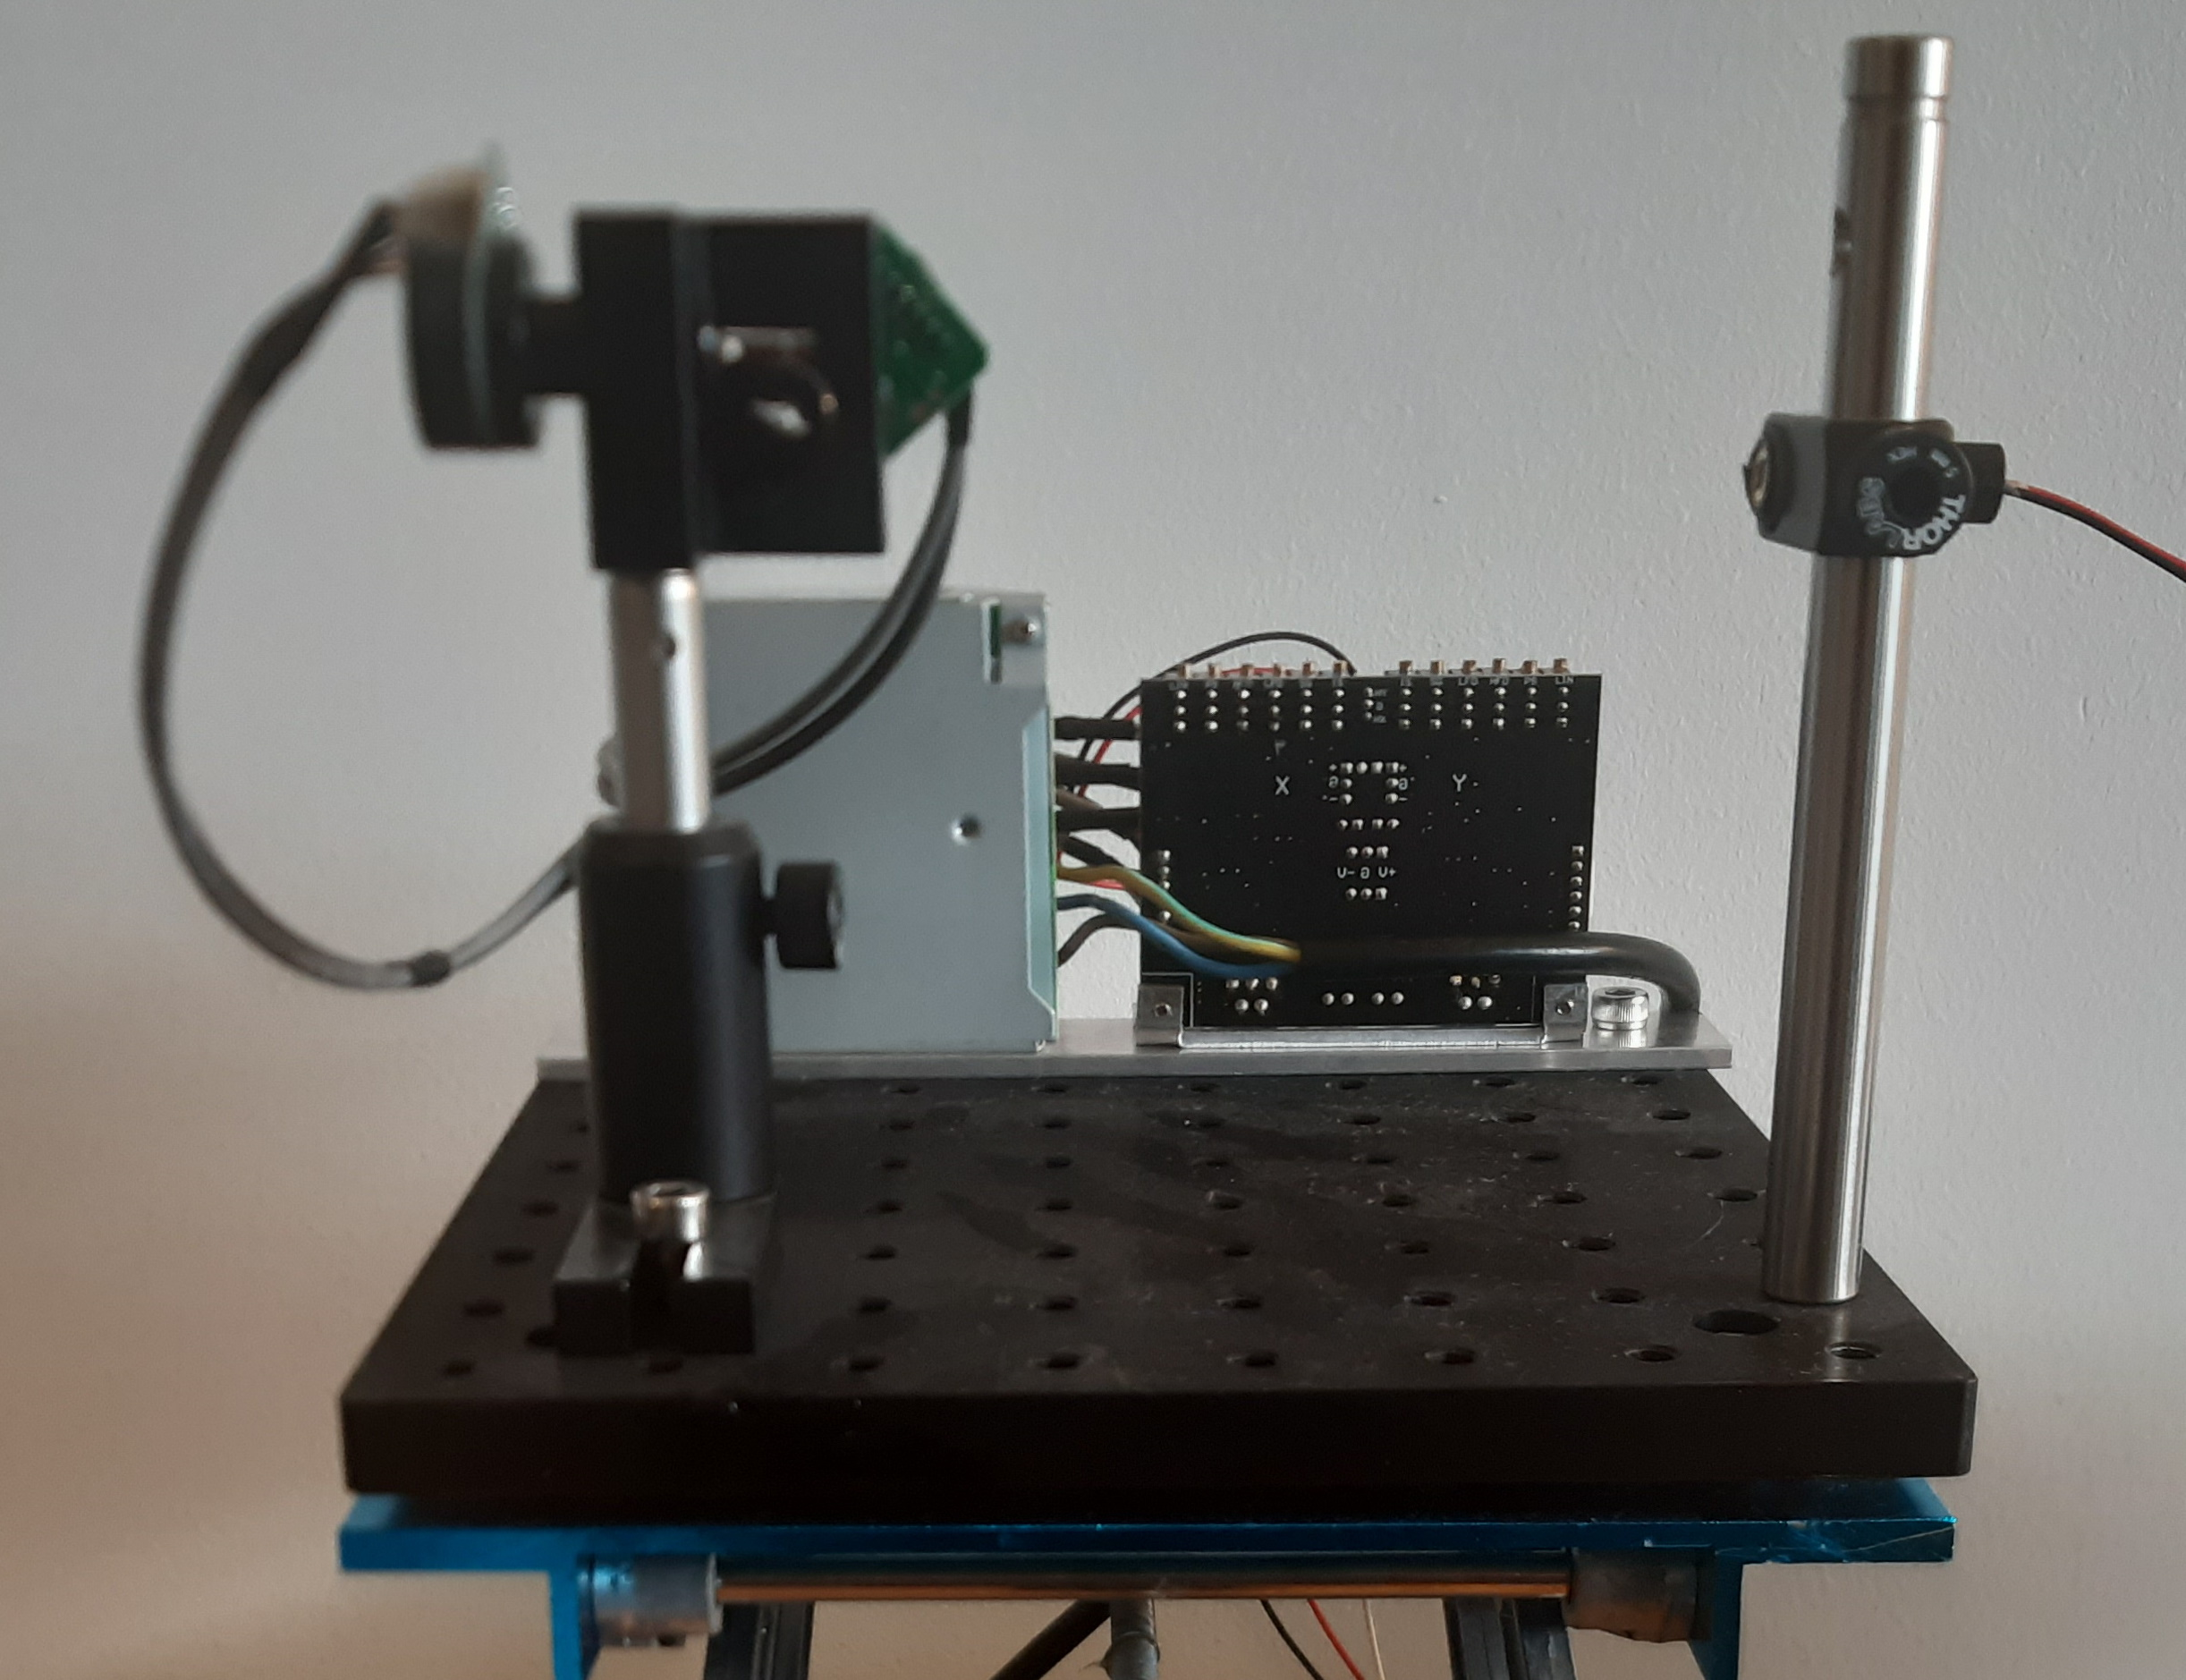
\includegraphics[width=\bildwidth]{pics/DutFront01.jpg}	\caption{DutFront01}	\label{DutFront01}	\end{figure}
% \begin{figure}[h!]	\centering	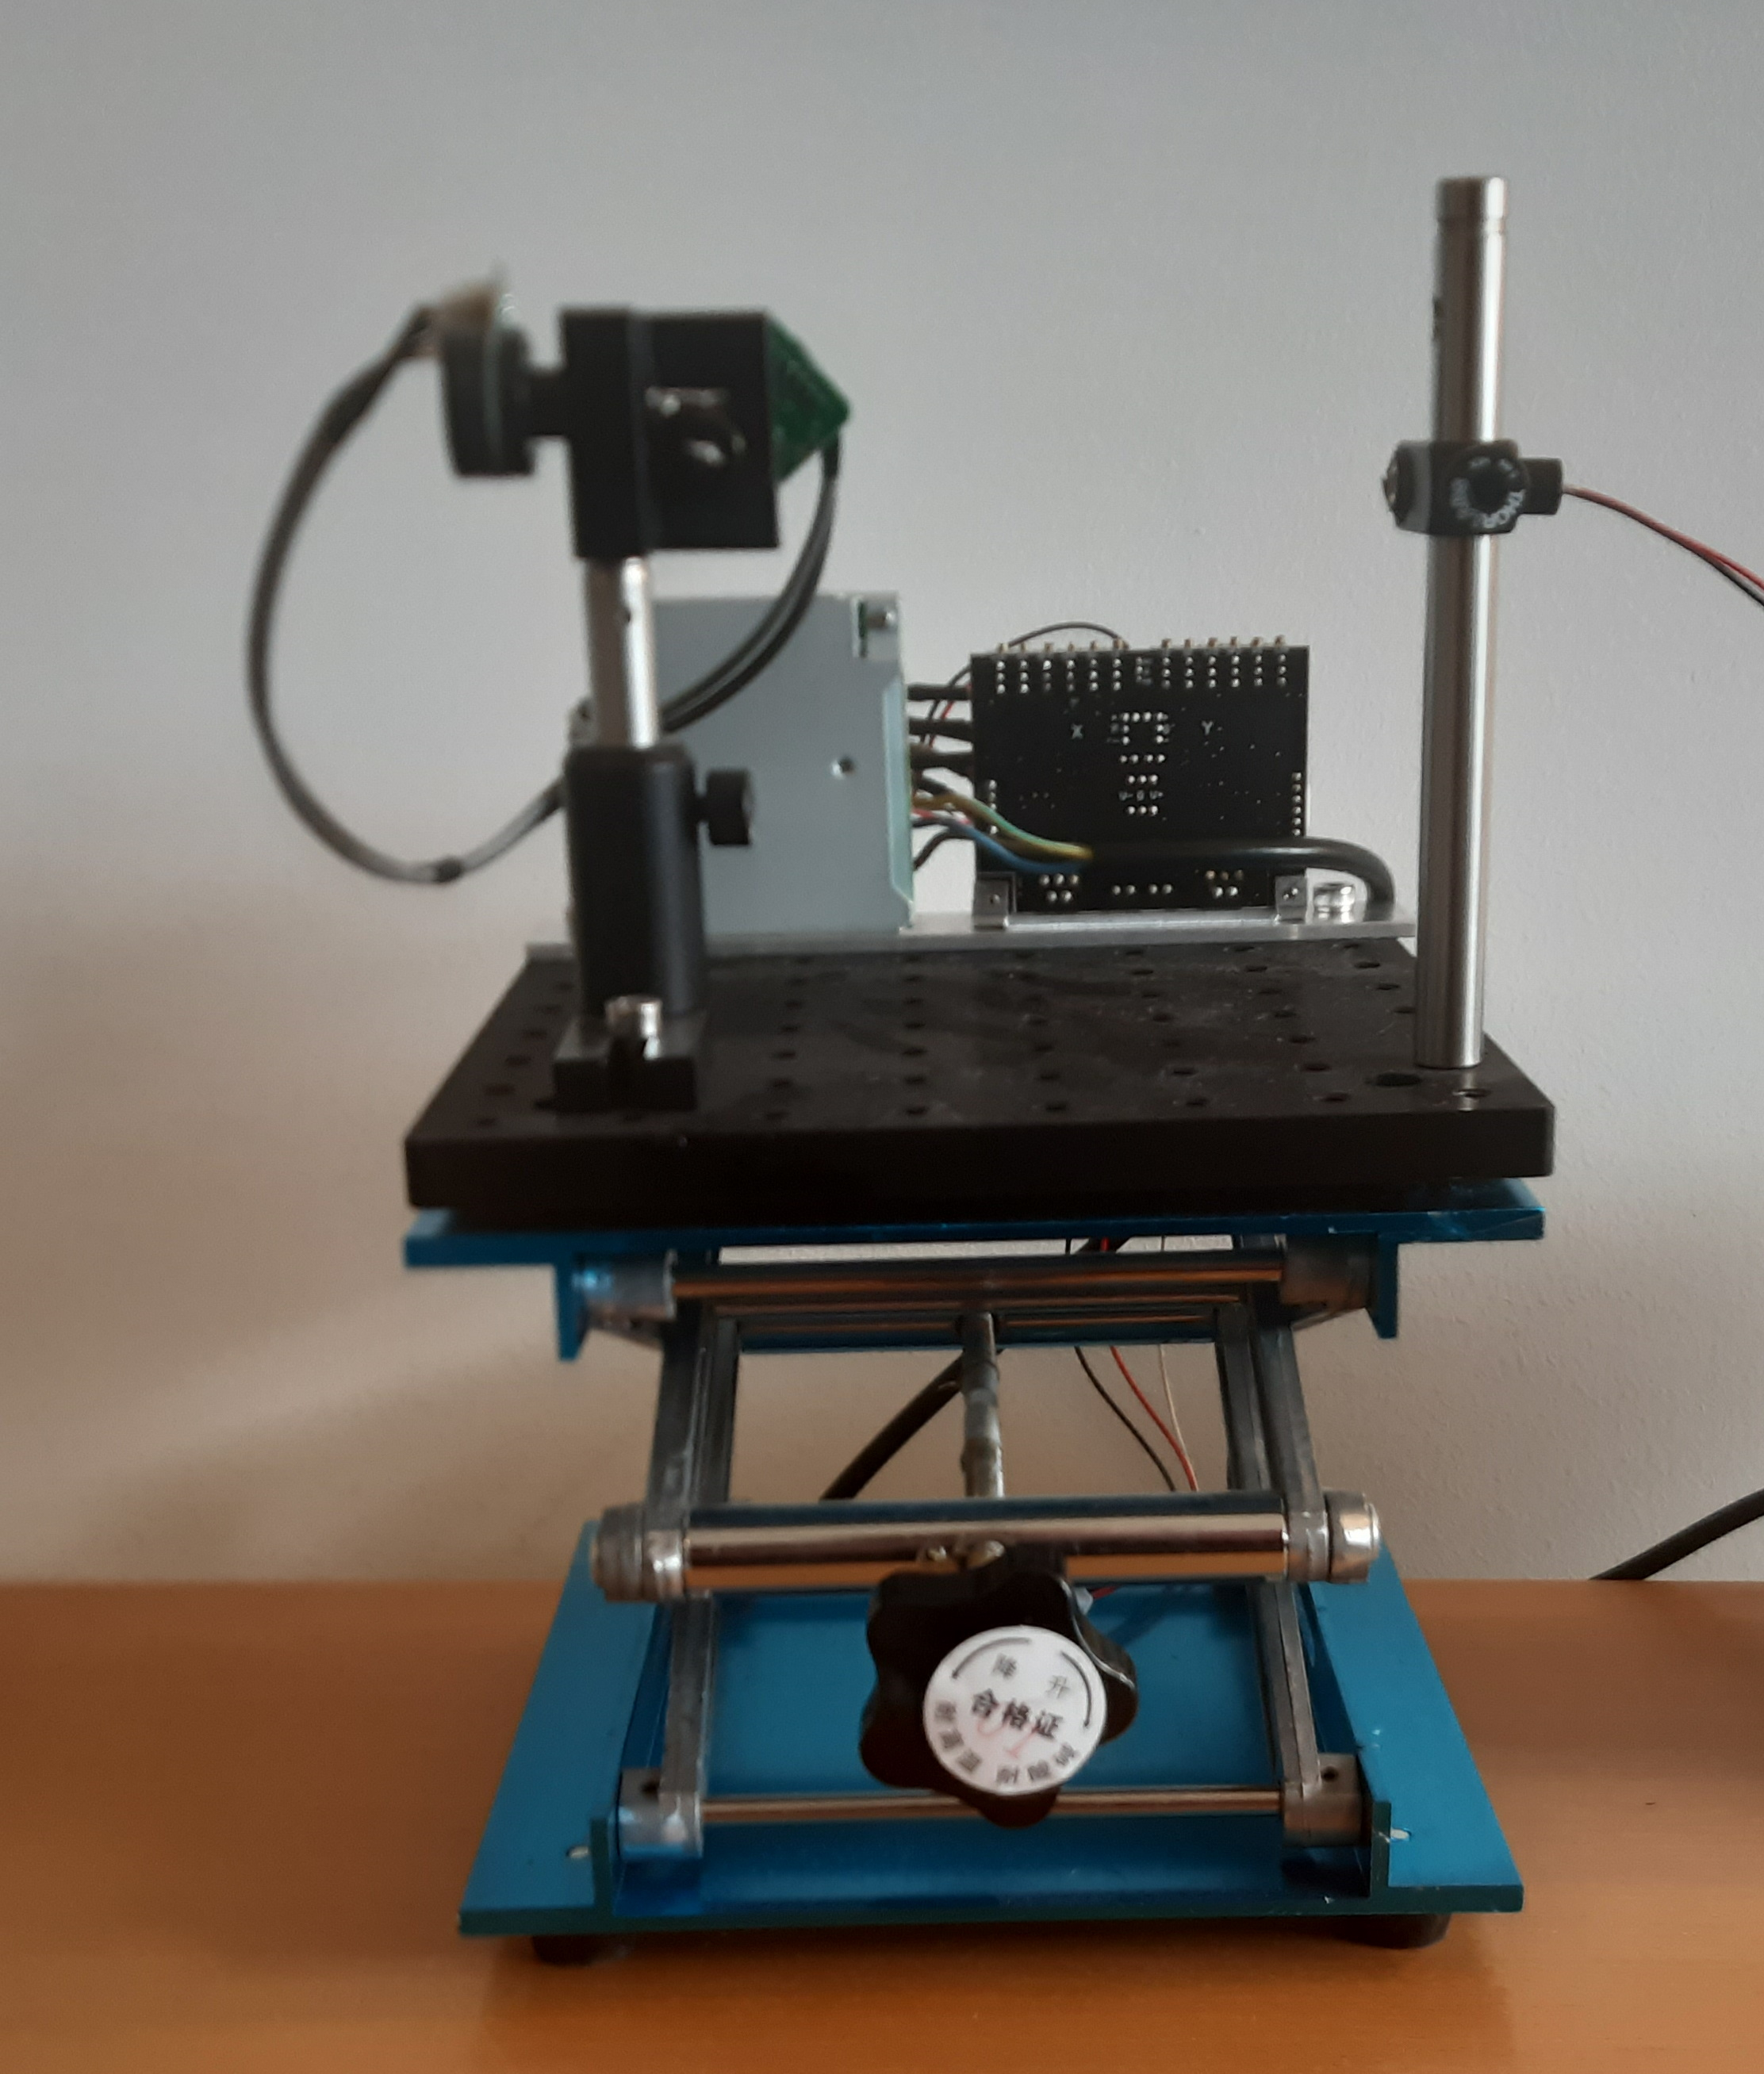
\includegraphics[width=\bildwidth]{pics/DutFront02.jpg}	\caption{DutFront02}	\label{DutFront02}	\end{figure}
% \begin{figure}[h!]	\centering	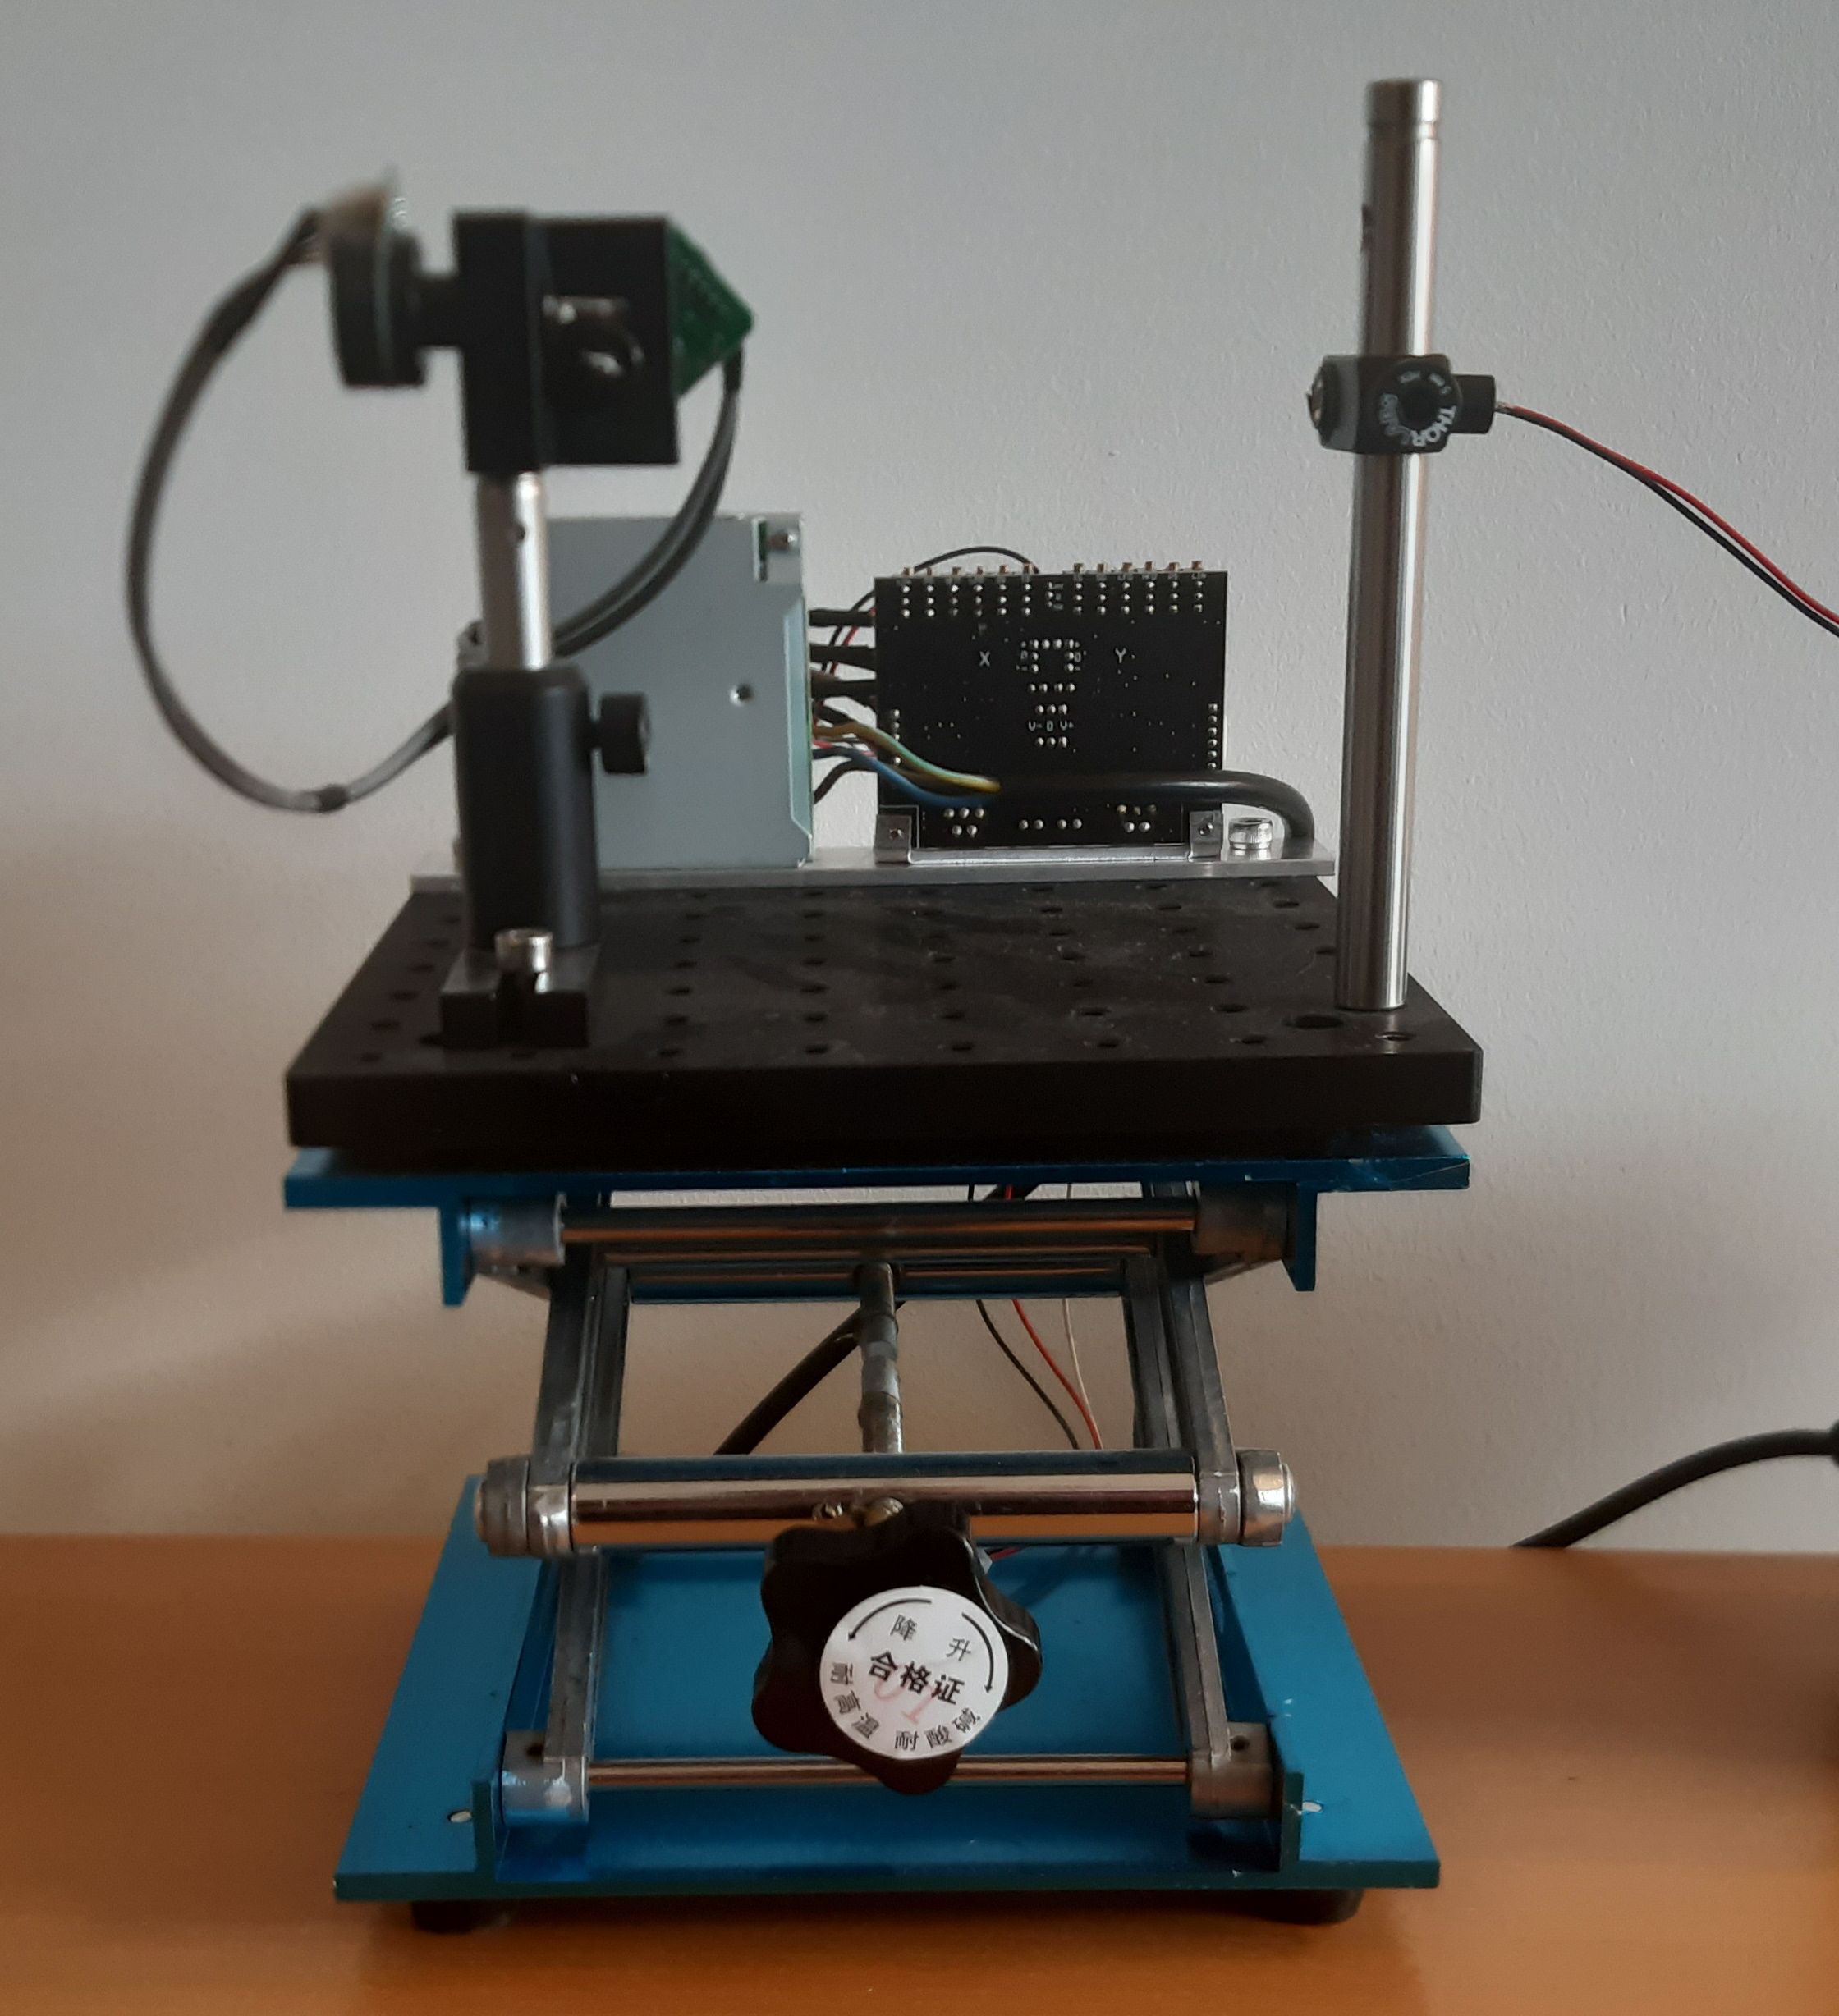
\includegraphics[width=\bildwidth]{pics/DutFront03.jpg}	\caption{DutFront03}	\label{DutFront03}	\end{figure}
% \begin{figure}[h!]	\centering	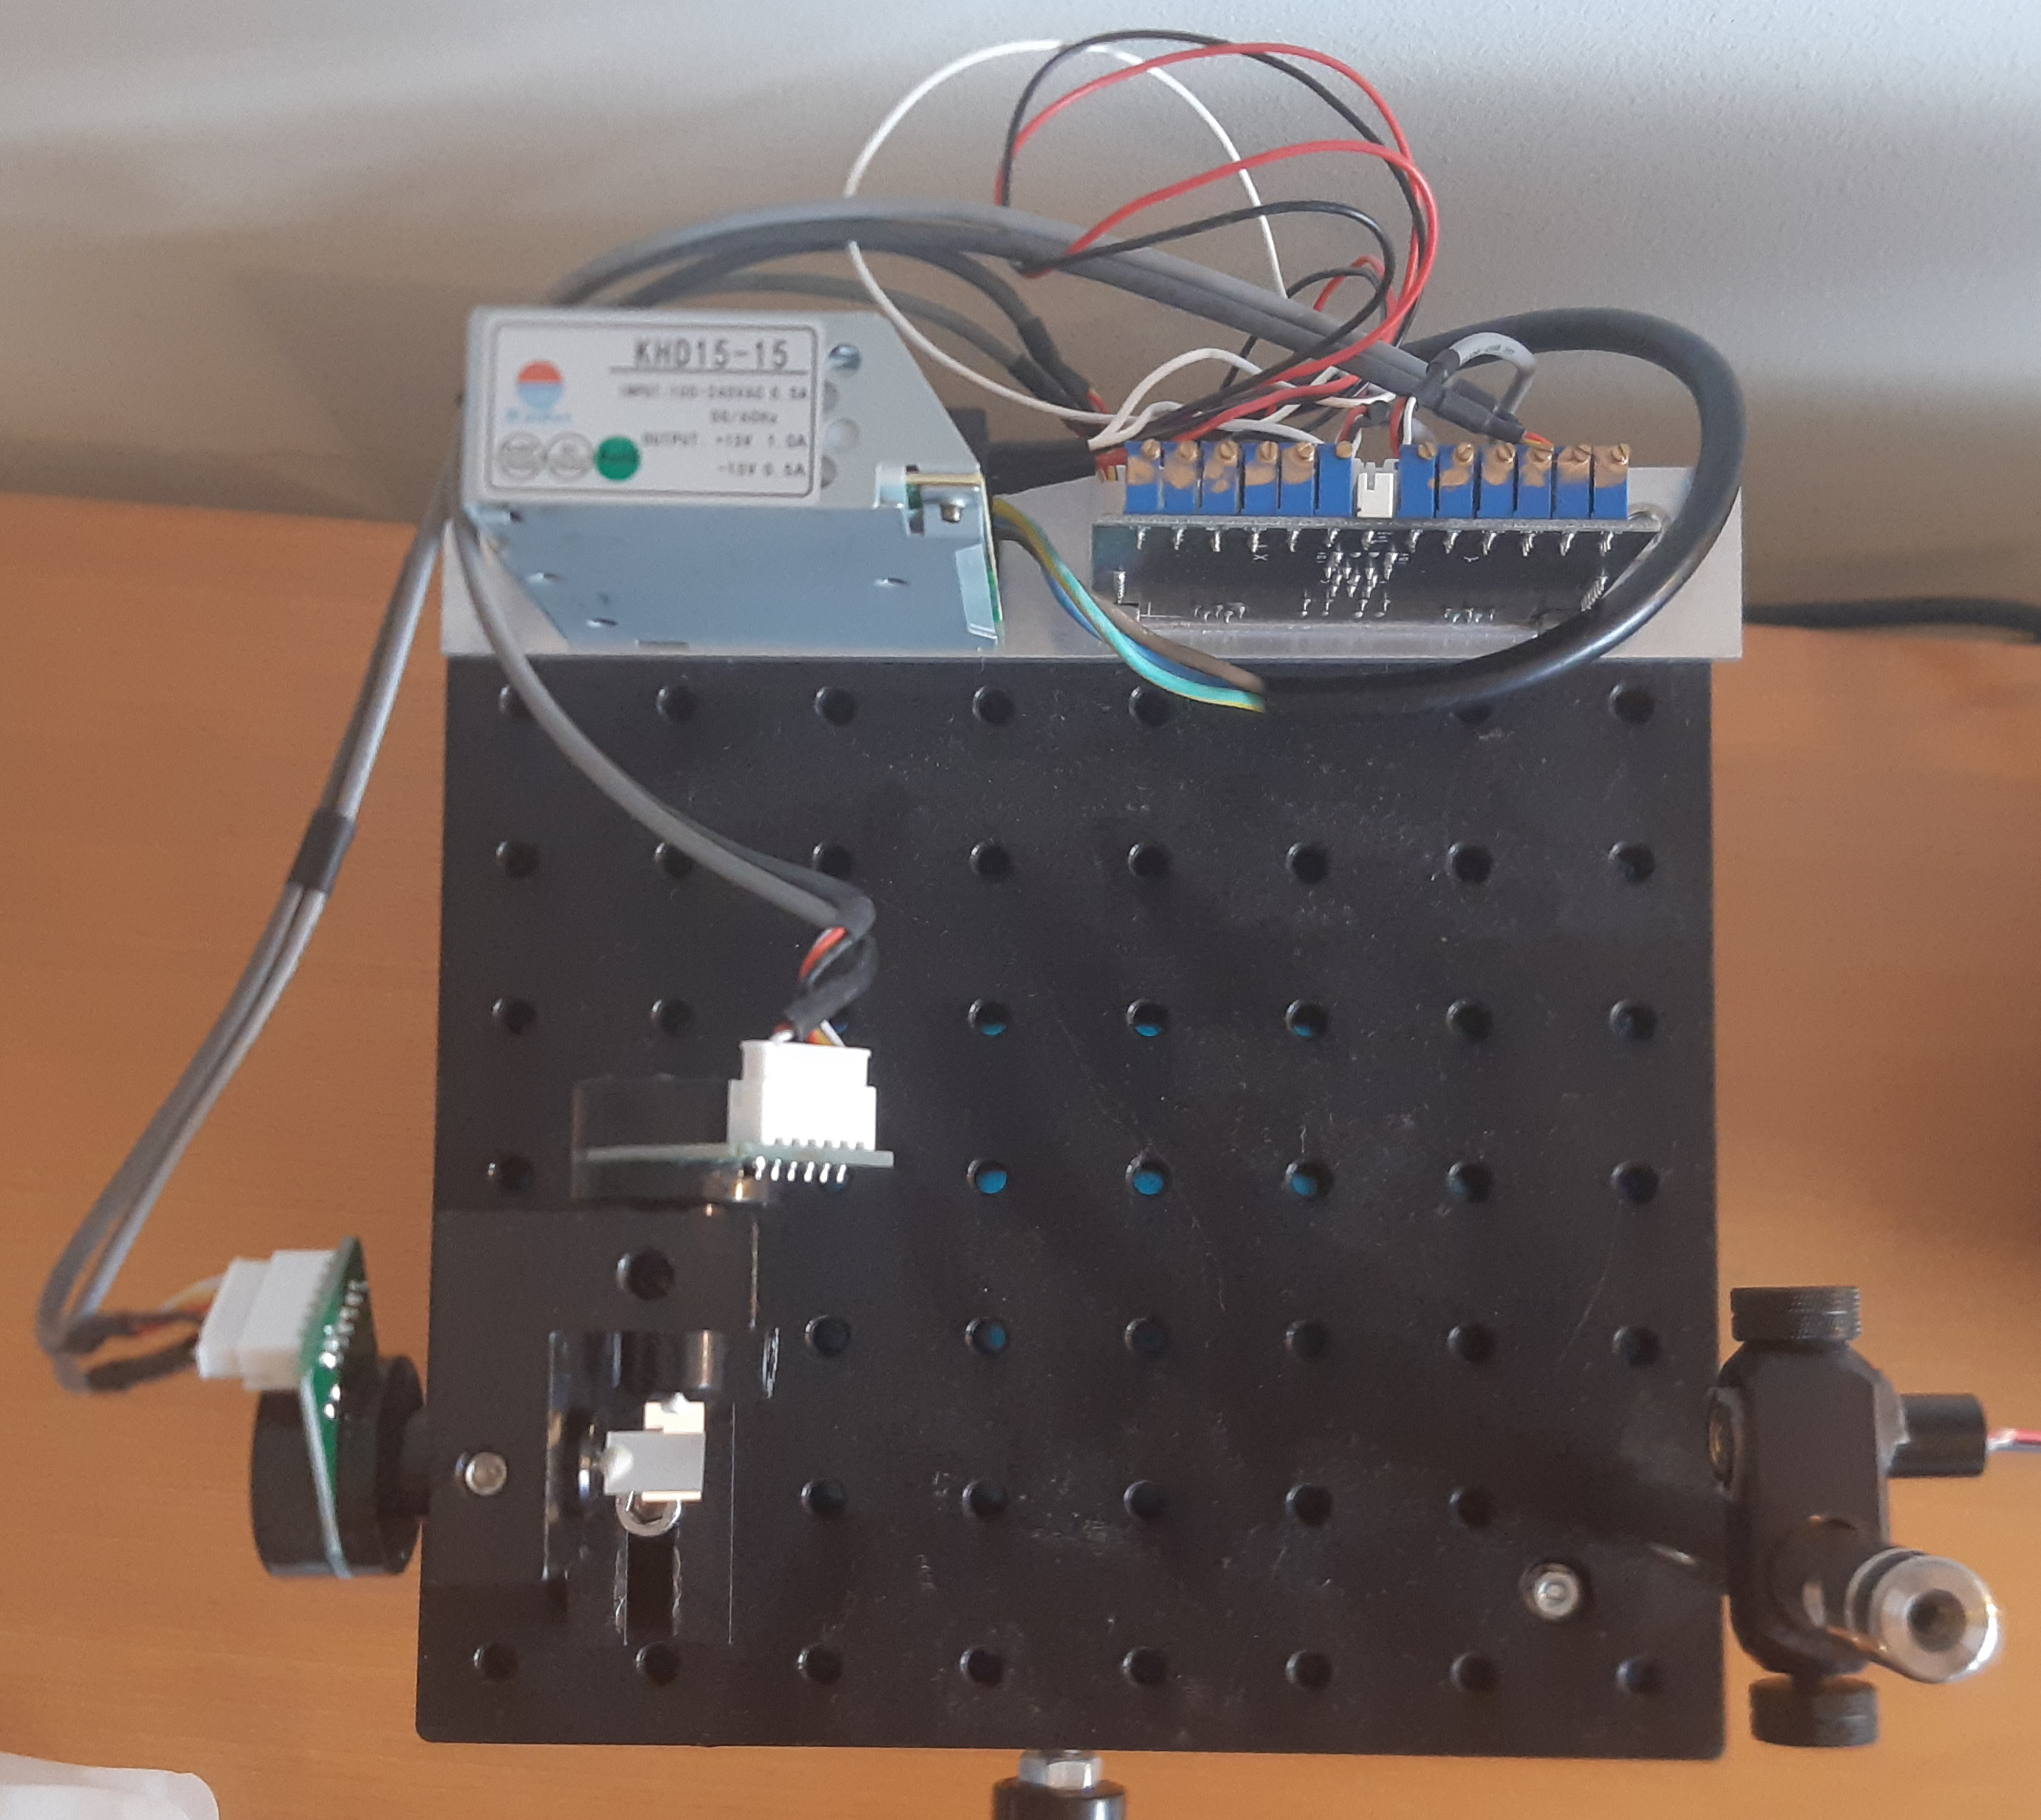
\includegraphics[width=\bildwidth]{pics/DutTop01.jpg}	\caption{DutTop01}	\label{DutTop01}	\end{figure}
\begin{figure}[h!]	\centering	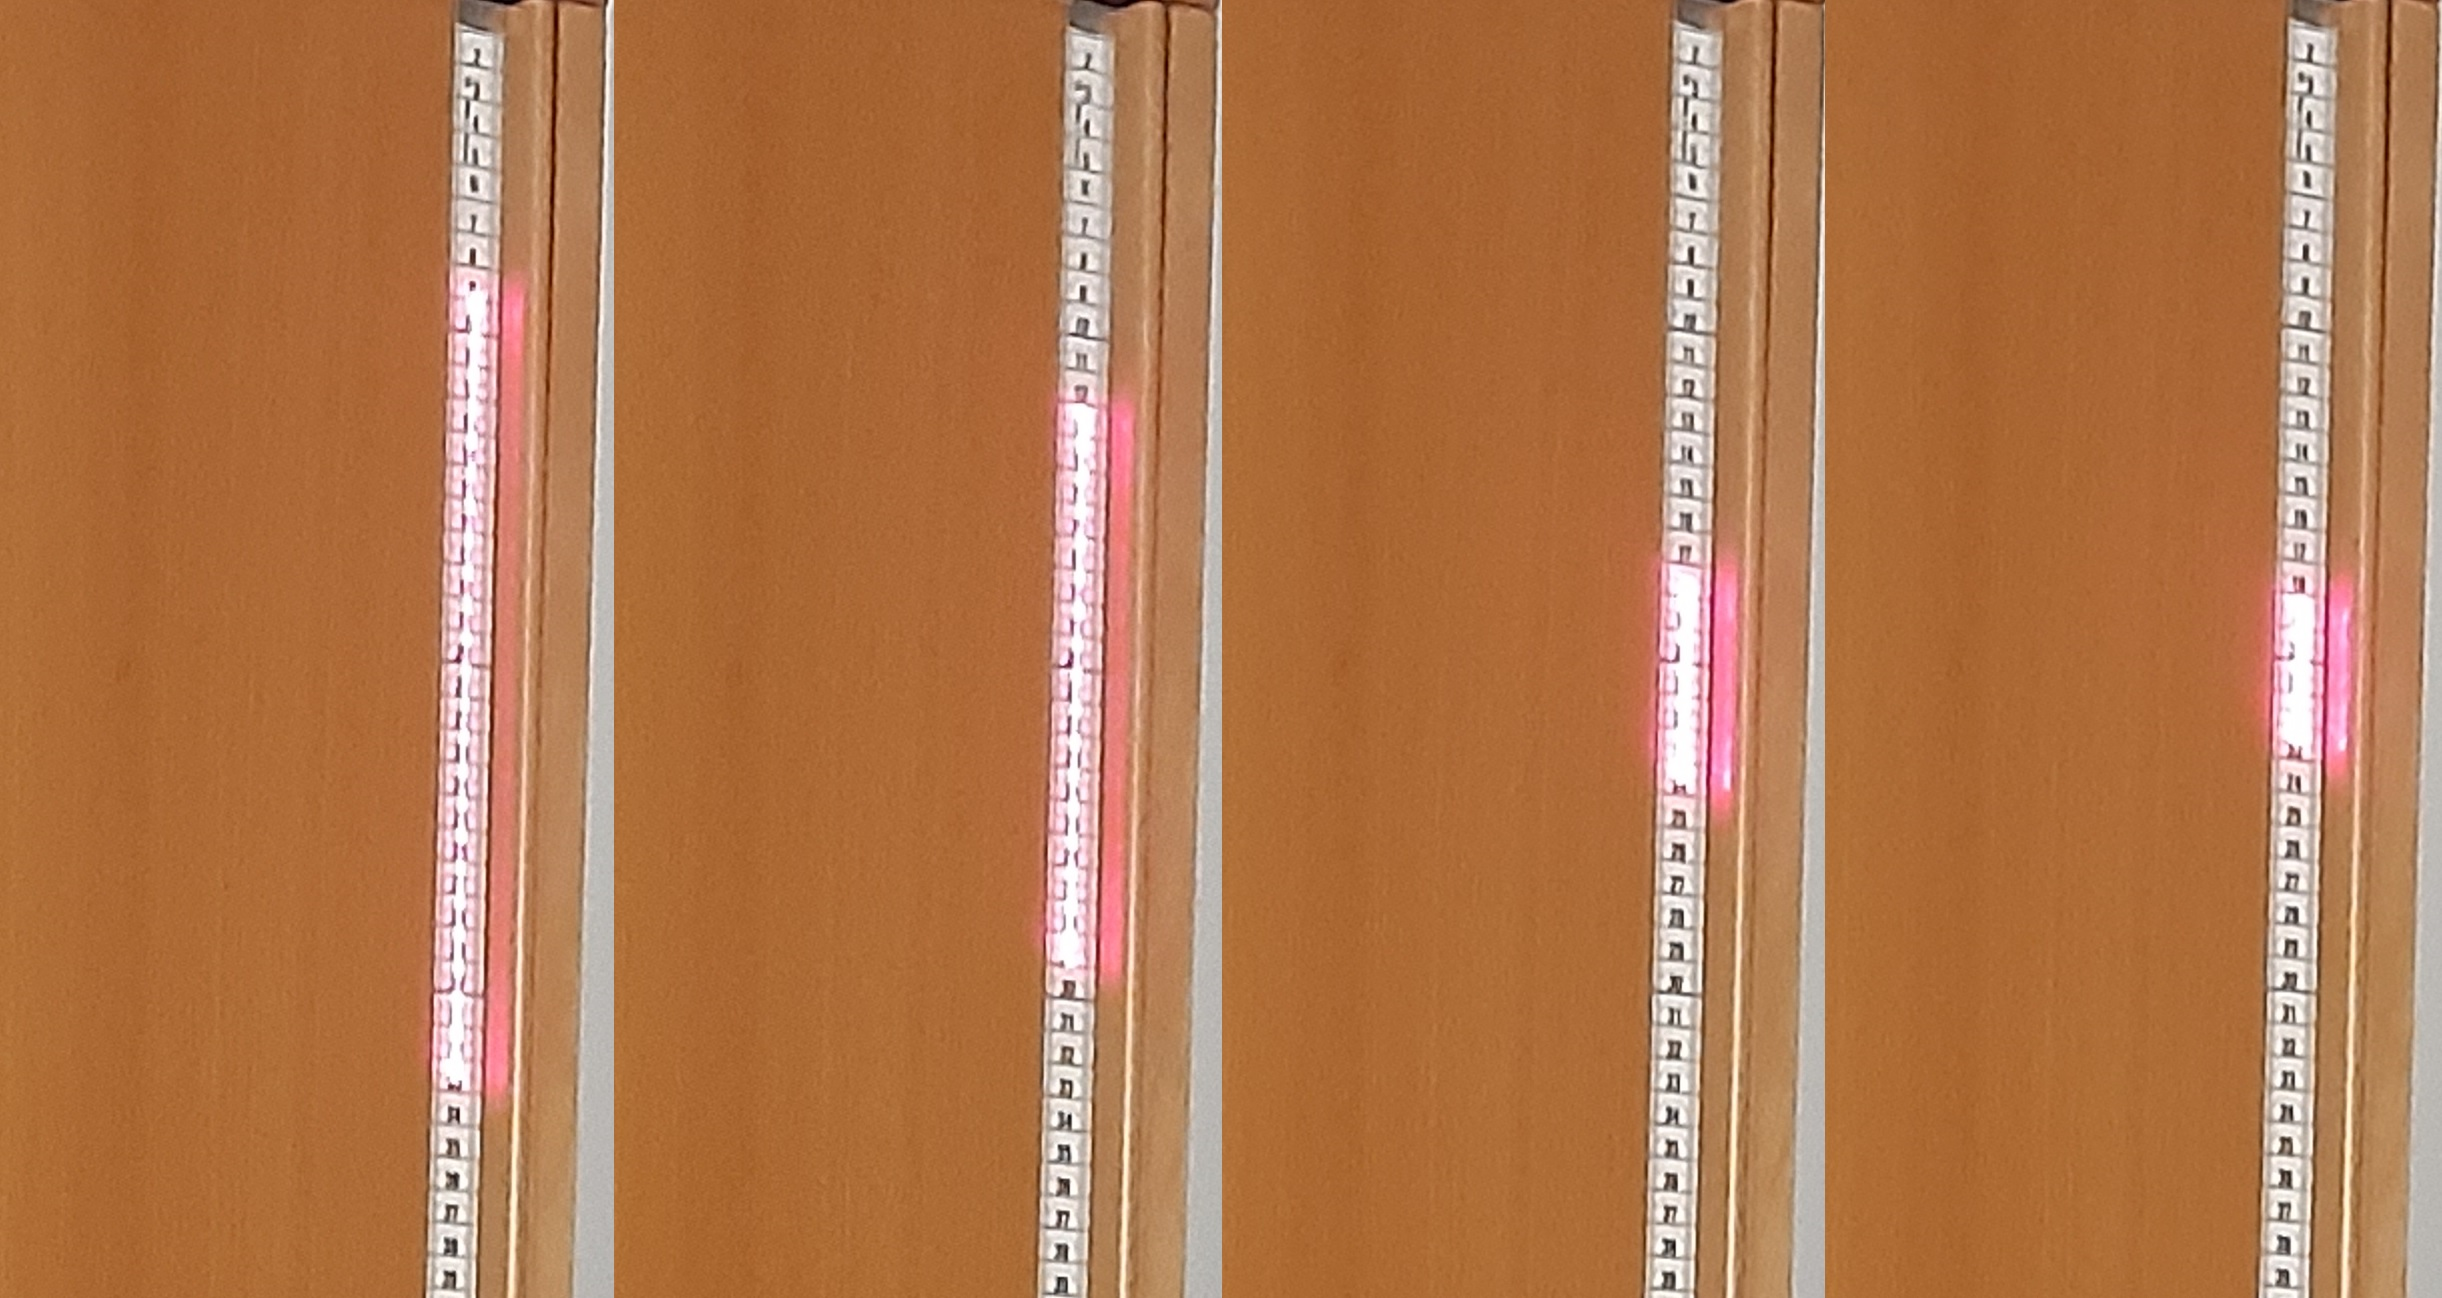
\includegraphics[width=\bildwidth]{pics/ImageMeasure01.jpg}	\caption{Abbilder von vier Messungen}	\label{ImageMeasure01}	\end{figure}
\bild{h!}{DetektorsForPhase}{Detektor zur Phasenmessung}{DetektorsForPhase}
% \begin{figure}[h!]	\centering	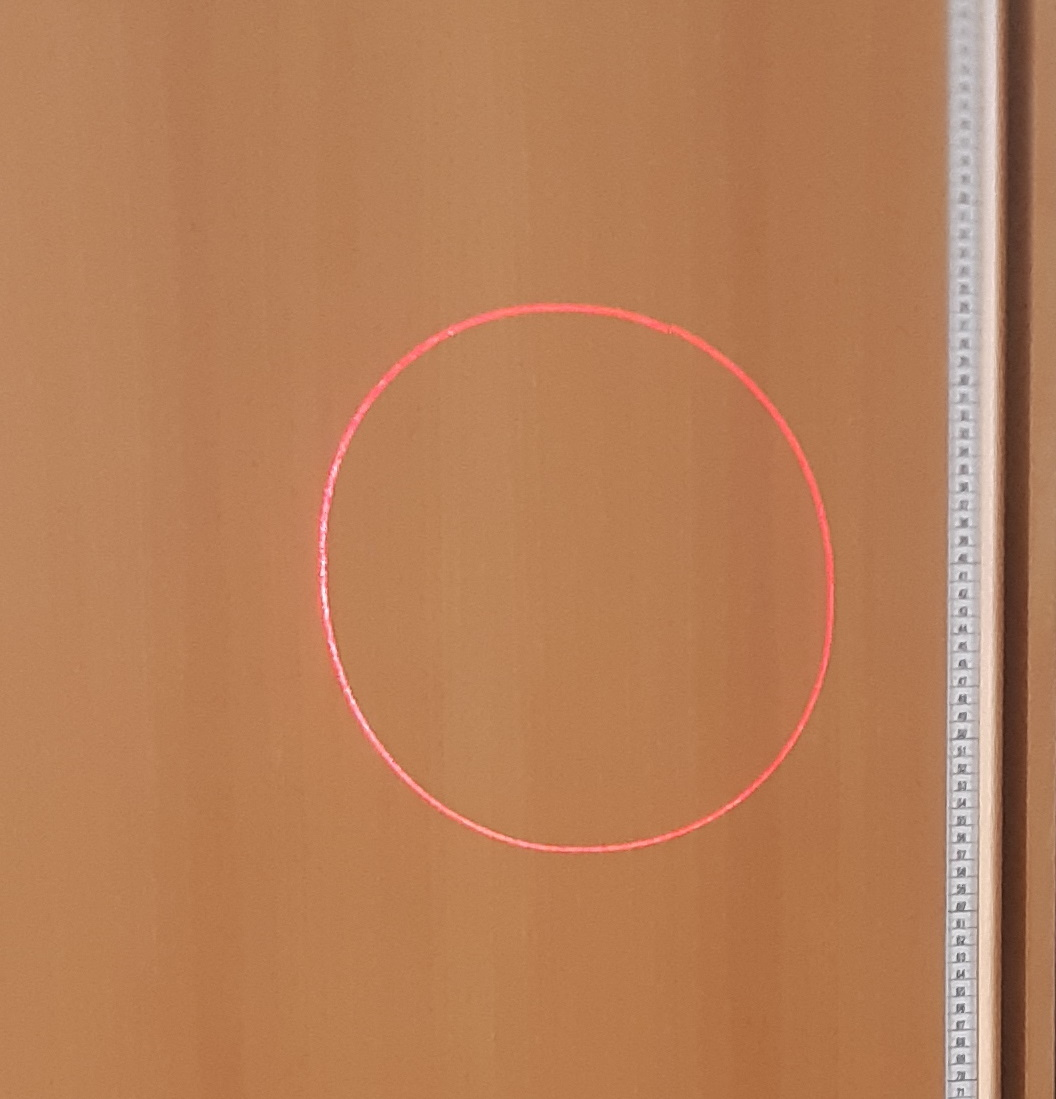
\includegraphics[width=\bildwidth]{pics/ImageXY01.jpg}	\caption{ImageXY01}	\label{ImageXY01}	\end{figure}
% \begin{figure}[h!]	\centering	\includegraphics[width=\bildwidth]{pics/.jpg}	\caption{}	\label{fig_sim}	\end{figure}

% \subsection{Messungen}
	% \begin{table}[h!]
	% \begin{center}
	% \begin{tabular}{l|l}
	% \input{Mess1.csv}
	% \end{tabular}
	% \caption{Messungcsv}
	% \label{Messungcsv}
	% \end{center}
	% \end{table}

\section{Ergebnisse}
\bild{h!}{Mess1log.eps}{Bode-Diagramm des \galvo }{Mess1log}
Die Ergebnisse der Messung sind in Abb.~\ref{Mess1log} dargestellt: Es existiert ein linearer Bereich unterhalb von 1kHz, bei dem die Auslenkung sehr exakt dem Steuersignal folgt. Oberhalb davon nimmt die Auslenkung mit steigender Frequenz ab und erreicht beim orangen Marker die -3dB-Grenzfrequenz mit 1.3kHz. Zwischen dem gruenen und roten Marker verdoppelt sich die Frequenz, was einer Oktave entspricht. Die Amplitude der Auslenkung faellt dabei um 6.43dB. Diese naeherungsweise 6dB/Oktave entsprechen 40dB/Dekade und somit einem System zweiter Ordnung der Form\cite{Staudecker}
	\begin{align*}
	% G(s) & = \frac{V}{(T_N s)^2 + 2 \xi T_N s +1} & \textrm{wird mit} \\
	% |s| & = |\alpha + j\omega| \overset{\alpha = 0} = \omega & \textrm{und} \\
	% T_N & = \frac{1}{\omega_0}  & 	\textrm{zu} \\
	G(\omega) & = \frac{V}{(\frac{\omega}{\omega_0} )^2 + 2 \xi \frac{\omega}{\omega_0}  +1} & \textrm{mit} \\
	% d &= 3190 mm \\
	\xi & = 1 \\
	\omega_0 &= 2\pi f_g \\
	f_{g}	& = 1300 Hz \\
	V &= 116.4 \frac{mm}{V} \\ % =  291mm/2.5V
	% dmax = 291mm
	% Vpp = 2.5V
	% f_{g,1Vpp} & = 1000 Hz \\
	\end{align*}
Die Daempfung $\xi$ mit '1' laesst sich aus dem Kurvenverlauf abschaetzen, da dieser keine Resonanzspitze an der Grenzfrequenz aufweist. Die Verstaerkung 'V' setzt die maximale Auslenkung mit der Amplitude der Steuerspannung ins Verhaeltnis. Auf eine Rueckrechnung von der Auslenkung auf den Drehwinkel des \galvo s wurde verzichtet. Fuer die Applikation ist die erreichbare Auslenkung in mm von Bedeutung, der Winkel stellt somit keine relevante Information dar. Beide vorhandenen  Galvanometer-Spiegel des Testobjektes wurden unter gleichen Bedingungen vermessen und zeigten nahezu identes Verhalten bezueglich ihrer Dynamik. Das Phasendiagramm ergibt sich mit der Formel \textrm{$\phi = 360^\circ f  \Delta t$} aus den gemessenen $\Delta t$. Diese wiederum stellen die Verzoegerung zwischen dem Nulldurchgang des Steuersignals, sowie der steigenden Flanke eines Opto-Detektors dar, der an der optischen Null-Position platziert ist. Der resultierende Verlauf entspricht einigermassen dem erwarteten Phasengang eines Systems 2ter Ordnung. Allerdings weist er schon bei tiefen Frequenzen eine Abweichung von der 0grad-Achse ab, was eine Totzeit des verwendeten Detektors vermuten laesst.
\section{Konklusion}
Das gewonnene Modell wird in einer Masterarbeit zur Adaptierung von Steuersignalen herangezogen. Das zugrundeliegende Konzept dazu nennt sich 'flachheitsbasierte Steuerung'. Hierbei wird das Steuersignal, unter Einbeziehung der Modell-Eigenschaften, so berechnet, dass der Ausgang einer Sollkurve folgt. Abgesehen von diesem direkten Nutzen der Messungen, verbessert sich auch das intuitive Verstaendnis der analysierten Komponenten und nuetzt damit bei der Applikation und Abschaetzung der Applizierbarkeit in OCT-Systeme. \\
Weitere Messungen mit unterschiedlichen Steuerspannungen und an mehreren Frequenzen, 	speziell im Bereich der Grenzfrequenz, sollen das bestehende Modell noch verfeinern. Auch soll die vermutete Totzeit des Opto-Detektors untersucht werden, damit praezisere Phasen-Messungen moeglich sind.

% \hfill rechtsbuendiger Text
\section*{Danksagung}
% \begin{itemize}
Martin Staudecker, Guenther Hannesschlaeger, Rankl Christian, Josef Langer und Silke Dorner, fuer die Assistenz bei Messungen.
% \end{itemize}
\label{cha:galvoChar}

% \chapter{Closing Remarks}
\label{cha:Closing}

%%%-----------------------------------------------------------------------------
\appendix                                                             % Appendix 
%%%-----------------------------------------------------------------------------

% \chapter{Technical Details}
\label{app:TechnicalDetails}



 % Technical supplements
\chapter{Supplementary Materials}
\label{app:materials}


List of supplementary data submitted to the degree-granting institution for archival storage
(in ZIP format).

% Use this as an example only, adapt the structure to your requirements!

\section{PDF Files}
\begin{FileList}{/}
\fitem{thesis.pdf} Master/Bachelor thesis (complete document)
\end{FileList}

\section{Media Files}
\begin{FileList}{/media}
\fitem{*.ai, *.pdf} Adobe Illustrator files
\fitem{*.jpg, *.png} raster images
\fitem{*.mp3} audio files
\fitem{*.mp4} video files
\end{FileList}


% \section{Online Sources (PDF Captures)}
% \begin{FileList}{/online-sources}
% \fitem{Reliquienschrein-Wikipedia.pdf} \parencite{WikiReliquienschrein2020}
% \end{FileList}




 % Contents of the CD-ROM/DVD
% \chapter{Questionnaire}
\label{app:Questionnaire}





 % Chronological list of changes
% \chapter{\latex Source Code}
\label{app:SourceCode}

 % Source text of this document

%%%-----------------------------------------------------------------------------
\backmatter                           % Back part (bibliography, glossary, etc.)
%%%-----------------------------------------------------------------------------

	\section{Abbreviations and Acronyms}
	\begin{table}[h!]
			\begin{tabular}{|p{2cm}|l|}
			\hline	
			uC		& MicroController							\\ \hline
			FW		& Firmware, the Software, running on the uC \\ \hline	
			OCT		& Optical Coherence Tomography				\\ \hline	
			SW		& Software, the Software, running on the OCT-System 	\\ \hline	
			FSM 	& Finite State Machine									\\ \hline
			CRC		& Cyclic Redundancy Check								\\ \hline
			IO		& Input-Output, bidirectional Communcation Lines 		\\ \hline
			USB		& Universal Serial Bus									\\ \hline
			VCP		& Virtual Com Port, a serial connection via USB			\\ \hline
			% CDC		& communications device class, implements VCP over USB	\\ \hline
			USB		& Universal Serial Bus									\\ \hline
			SCPI	& Standard Commands for Programmable Instruments, as defined by IEEE 488.2	\\ \hline
			% r.SCPI	& RECENDTs adaption of SCPI, employed for Communication between SW and FW	\\ \hline
			LUT		& Look-up-table											\\ \hline
			IRQ		& Interrupt request										\\ \hline
			ISR		& Interrupt-service-routine, a function within the FW, that is called by an IRQ	\\ \hline
			HW		& Hardware, the entirety of uC, the PCB and peripherals	\\ \hline
			SLD		& Super luminiscence Diode								\\ \hline
			AIM		& Aiming Laser											\\ \hline
			CAM		& Camera												\\ \hline
			LED		& Light emitting diode									\\ \hline
			LSB		& Least significant bit									\\ \hline
					% & \\ \hline
					% & \\ \hline
			\end{tabular}
			\caption{Abbreviations}
		\end{table}


\MakeBibliography % References

%%%-----------------------------------------------------------------------------
% Special page for checking print size
%%%-----------------------------------------------------------------------------

% \chapter*{Check Final Print Size}

\begin{center}
{\Large --- Check final print size! ---}

\bigskip

\calibrationbox{100}{50} % width/height of box in mm

\bigskip

{\Large --- Remove this page after printing! ---}

\end{center}



%%%-----------------------------------------------------------------------------
\end{document}
%%%-----------------------------------------------------------------------------
